\documentclass[12pt]{cmuthesis}

%for a more compact document, add the option openany to avoid
%starting all chapters on odd numbered pages

\usepackage{comment}
% \usepackage[ruled,vlined]{algorithm2e}
\usepackage[boxed,ruled,vlined,figure]{algorithm2e}
\usepackage[utf8]{inputenc} % usually not needed (loaded by default)
\usepackage[T1]{fontenc}
\usepackage{url}
\usepackage{ifthen}
\usepackage{framed}
\usepackage{enumitem}
\usepackage{multirow}
\usepackage{subcaption}
\usepackage{times}
\usepackage{amssymb}
\usepackage[export]{adjustbox}
\usepackage{rotating}
\usepackage{times}
\usepackage{fullpage}
\usepackage{amsmath}
\usepackage[numbers,sort]{natbib}
\usepackage[pagebackref,pageanchor=true,plainpages=false, pdfpagelabels, bookmarks,bookmarksnumbered]{hyperref}
%pdfborder=0 0 0,  %removes outlines around hyper links in online display
% \usepackage{subfigure}
\usepackage{color}
\usepackage{soul}
\usepackage{xspace}
\usepackage{makecell}
\usepackage{booktabs}
\usepackage{graphicx}
\usepackage{epsfig}
\usepackage{siunitx}
\usepackage{listings}
\usepackage[]{algorithm2e}
\usepackage{float}

\lstset{
    frame=single,
    framexleftmargin=15pt
}

%% paramgraph

\setlength{\parskip}{6pt}

%%%
%%%  Comments
%%%
\newcommand{\showComments}{yes}
\newcommand{\note}[2]{
    \ifthenelse{\equal{\showComments}{yes}}{\textcolor{#1}{#2}}{}
}

\newcommand{\showRevision}{no}
\newcommand{\revision}[1]{
    \ifthenelse{\equal{\showRevision}{yes}}{\textcolor{red}{#1}}{#1}
}


\newcommand{\TODO}[1]{\note{red}{#1}}


% FOR SUBMISSION ONLY: Eliminate copyright box at bottom of first page
% Use \toappear{} if you want a blank ACM copyright box instead of suppressing it
\usepackage{etoolbox}
\makeatletter
\patchcmd{\maketitle}{\@copyrightspace}{}{}{}
\makeatother


% Itemize and Enumerate with less white space wasted
\newenvironment{smitemize}%
{\begin{list}{$\bullet$}%
        {\setlength{\parsep}{1pt}%
        \setlength{\topsep}{1pt}%
        \setlength{\itemsep}{1pt}}}%
              {\end{list}}

\newenvironment{smenumerate}{
    \begin{enumerate}
        \setlength{\itemsep}{2.5pt}
              \setlength{\parskip}{0pt}
              \setlength{\parsep}{0pt}
              }{\end{enumerate}}

\newenvironment{mypara}{
    \vspace{0.1in}
    \textbf}
{\plain}


\newcommand{\lc}[1]{\lowercase{#1}}
\newcommand{\uc}[1]{\uppercase{#1}}
\newcommand{\xc}[1]{\small\sc #1}


\newenvironment{captiontext}{%
    \par\vspace{0.1in}\renewcommand{\baselinestretch}{0.9}}%
{\renewcommand{\baselinestretch}{1.0}\par}


%
% defining the \BibTeX command - from Oren Patashnik's original BibTeX documentation.
\def\BibTeX{{\rm B\kern-.05em{\sc i\kern-.025em b}\kern-.08emT\kern-.1667em\lower.7ex\hbox{E}\kern-.125emX}}

\usepackage{setspace} % for \onehalfspacing and \singlespacing macros
\usepackage{etoolbox}
\AtBeginEnvironment{quote}{\singlespacing\small}

% \settopmatter{printacmref=false} % Removes citation information below abstract
% \renewcommand\footnotetextcopyrightpermission[1]{} % removes footnote with conference information in first column
% \pagestyle{plain}


% Abbreviations


% Approximately 1" margins, more space on binding side
%\usepackage[letterpaper,twoside,vscale=.8,hscale=.75,nomarginpar]{geometry}
%for general printing (not binding)
\usepackage[letterpaper,twoside,vscale=.8,hscale=.75,nomarginpar,hmarginratio=1:1]{geometry}

% Provides a draft mark at the top of the document.
% \draftstamp{\today}{DRAFT}

%\includeonly{synthetic}

\begin{document}

%\frontmatter

\title{{\bf Scaling Up Wearable Cognitive Assistance for Assembly Tasks}}
\author{Roger Iyengar \\ \href{mailto:raiyenga@cs.cmu.edu}{raiyenga@cs.cmu.edu}}
\date{December 2022}
\Year{2022}
\trnumber{}

\vspace{3cm}

\committee{
  Mahadev Satyanarayanan (Satya) (Chair) \\
  Martial Hebert \\
  Roberta Klatzky \\
  Padmanabhan Pillai (Intel Labs)
}

\support{
  This work was supported by an NSF Graduate Research Fellowship under Grants
  DGE1252522 and DGE1745016.
}
% \disclaimer{}

% copyright notice generated automatically from Year and author.
% permission added if \permission{} given.

%\keywords{}

%\maketitle

% \begin{dedication}

% \end{dedication}

%% Obviously, it's probably a good idea to break the various sections of your thesis
%% into different files and input them into this file...

% \begin{abstract}

% \end{abstract}

% \begin{acknowledgments}

% \end{acknowledgments}

% \tableofcontents
% \listoffigures
% \listoftables
\mainmatter

%% Double space document for easy review:
%\renewcommand{\baselinestretch}{1.66}\normalsize

% The other requirements Catherine has:
%
%  - avoid large margins.  She wants the thesis to use fewer pages,
%    especially if it requires colour printing.
%
%  - The thesis should be formatted for double-sided printing.  This
%    means that all chapters, acknowledgements, table of contents, etc.
%    should start on odd numbered (right facing) pages.
%
%  - You need to use the department standard tech report title page.  I
%    have tried to ensure that the title page here conforms to this
%    standard.
%
%  - Use a nice serif font, such as Times Roman.  Sans serif looks bad.
%
% Other than that, just make it look good...

\chapter{Detecting Completed Steps}\label{chap:detection}

A WCA applications for a physical assembly task must detect when a step of the
task has been completed.
A user wears a mobile device with a camera (such as a Google Glass).
The mobile
device gives the user an instruction, waits for them to complete this, and then
gives them the next instruction.
Completing a step might require adding a part to the assembly,
removing a part from the assembly, or repositioning the object in order to give
the camera a certain view.
The application must determine when a step is completed
based on images from the camera.
It is important to avoid false positives, which are instances where the
application determines that a step has been completed before it actually has
been.
False positives cause the application to give the user a new instruction before
the previous step gets completed, which results in a poor user experience.

\section{Hierarchical Decomposition}

An object made up of many parts is going to be larger than most of the
individual parts.
Rather than asking the user to move their head close to each part
they install, the system should be able to determine when a step has been
completed based on an image that contains most or all of the full object being
assembled.
Breaking up a large object into a collection of sub-assemblies makes
this possible.
Our system uses a two stage process where it first finds the
region of an image that contains the sub-assembly involved in a step. It then
crops the image around this region, and the next model determines if the step
has been completed based on the cropped image. Inspired by Simon's argument that
all complex systems are made up of smaller systems~\cite{Simon1991}, we argue
that any object that is assembled from more than ten parts can be decomposed
into sub-assemblies.
Hence the hierarchical approach proposed here can be scaled upwards, without
obvious limits.

This technique is applicable to tasks
with multiple levels of sub-assembly hierarchies.
An assistant for a task involving multiple sub-assemblies is effectively a
series of independent applications. Once the user completes one sub-assembly,
they will automatically be taken to the assistant for the next one.
If the
sub-assemblies must be connected together after that, there will be an assistant
for these steps as well.
Tasks can be broken into sub-assemblies the same way that long documents can be
broken into chapters, sections, and subsections.
Sub-assemblies near the top of the hierarchy are going to be made up of multiple
levels of sub-assemblies below them.

Figure~\ref{fig:stirling_full} shows two of the sub-assemblies of a Stirling
engine.
Our application uses a different pair of computer vision models for each
sub-assembly.
The code selects the correct pair based on the current step that the user is
working on.
Each step involves removing a piece from one sub-assembly.
None of the sub-assemblies involve more than 8 steps.
Splitting the task up into sub-assemblies thus simplifies the scope of the
problem to developing a set of assistants for 8 step tasks.

The number of steps required for each sub-assembly is not something that we have
any fixed rules about. We have found that limiting the number of steps to 10
appears to work well empirically, but the optimal number of steps for a
sub-assembly will likely vary based on the task.

\begin{figure}

  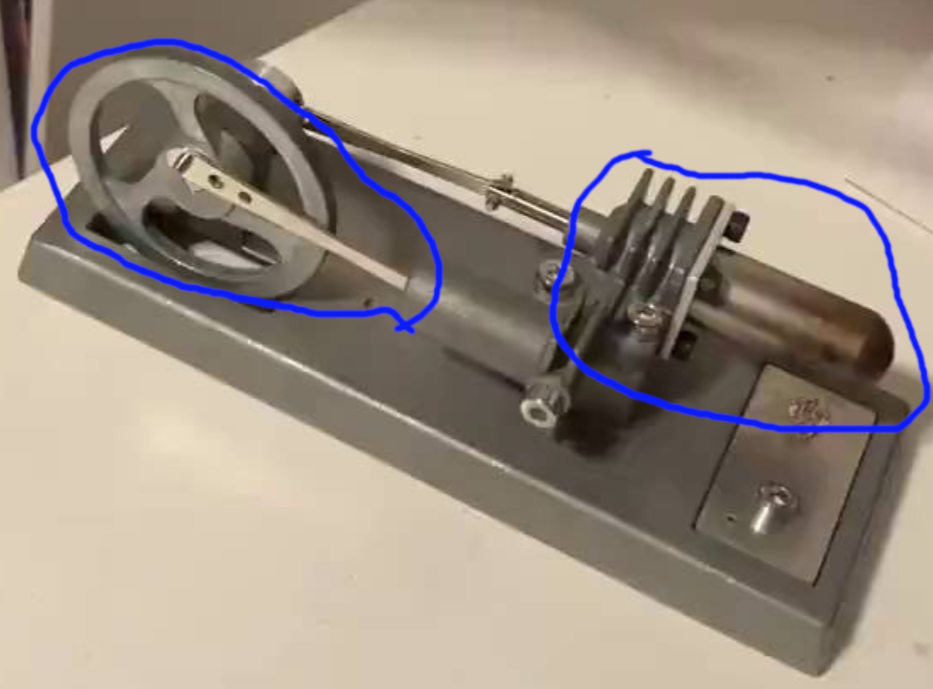
\includegraphics[width=7cm]{figures/stirling/full.png}
  \caption{A stirling engine with two sub-assemblies highlighted
  }\label{fig:stirling_full}
\end{figure}

Figure~\ref{fig:erector} shows how a model motorcycle can be broken up into
three sub-assemblies.
The Stirling engine has a single large base, but the motorcycle is simply
assembled from small pieces. Therefore, assembling the motorcycle would require
an additional set of steps at the end, to connect the sub-assemblies together.

\begin{figure}
  \begin{subfigure}{\textwidth}
    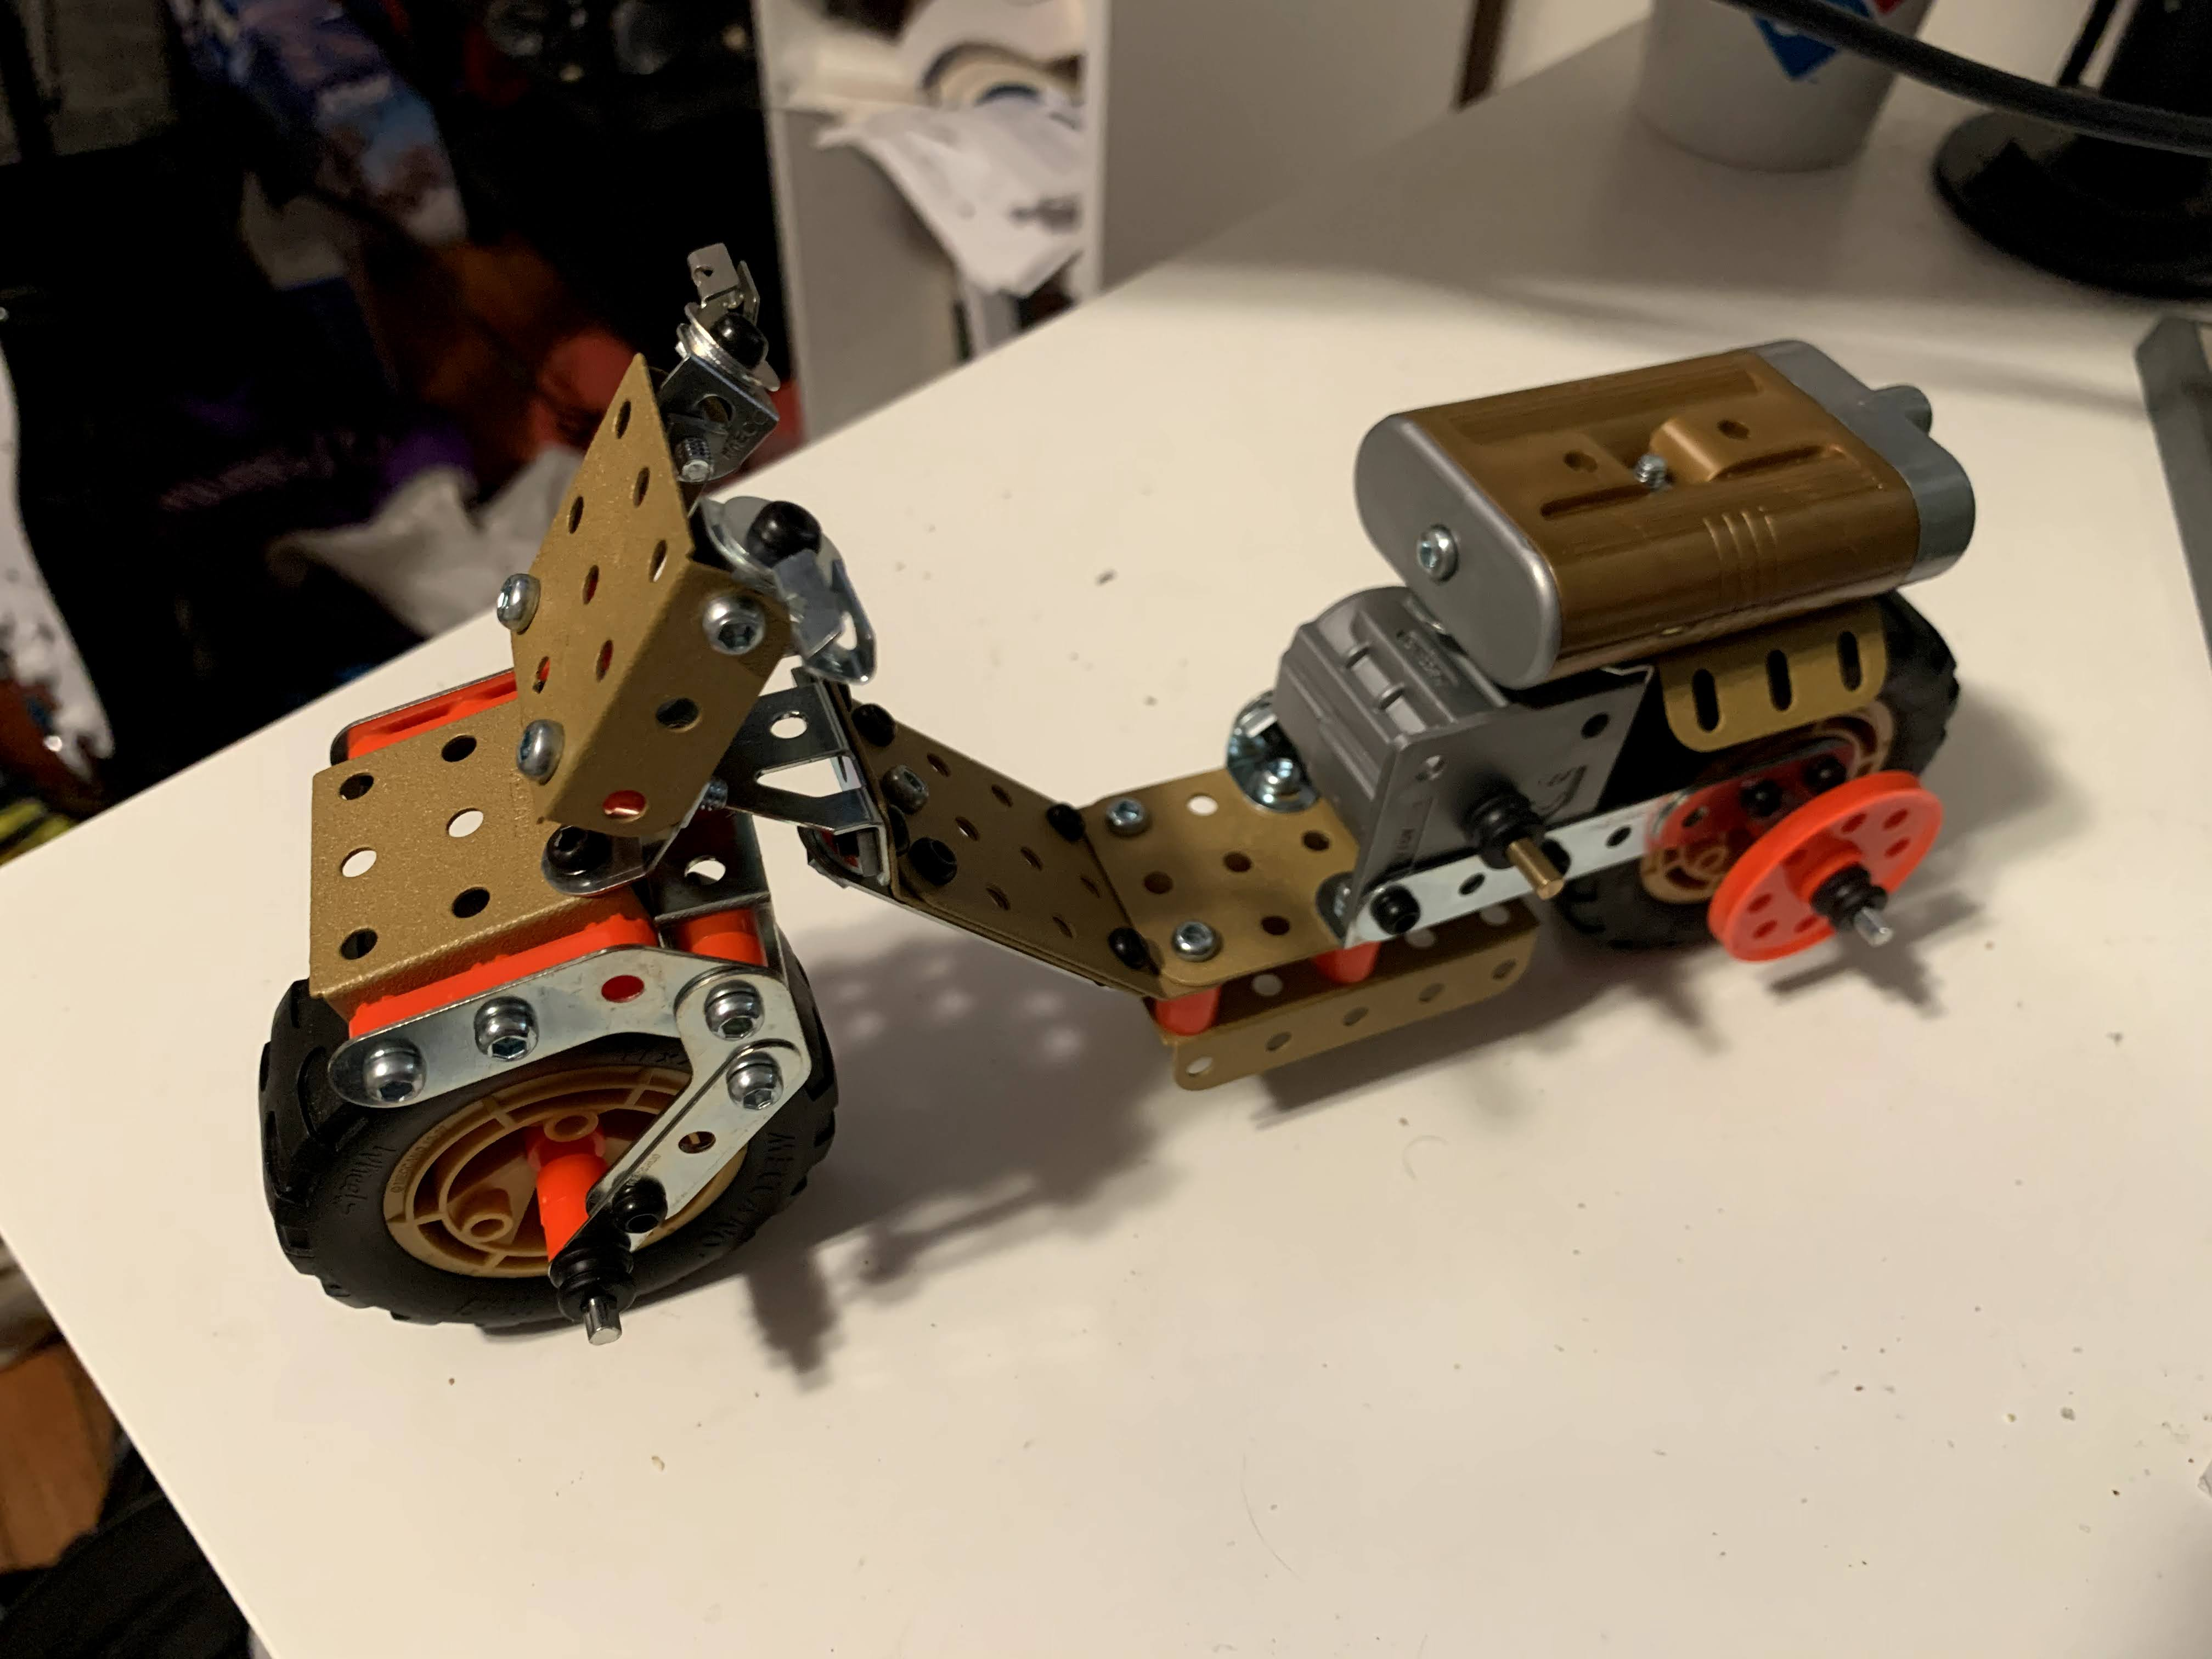
\includegraphics[width=5cm]{figures/erector/full.jpg}
    \caption{The fully-assembled model}
  \end{subfigure}
  \begin{subfigure}{\textwidth}
    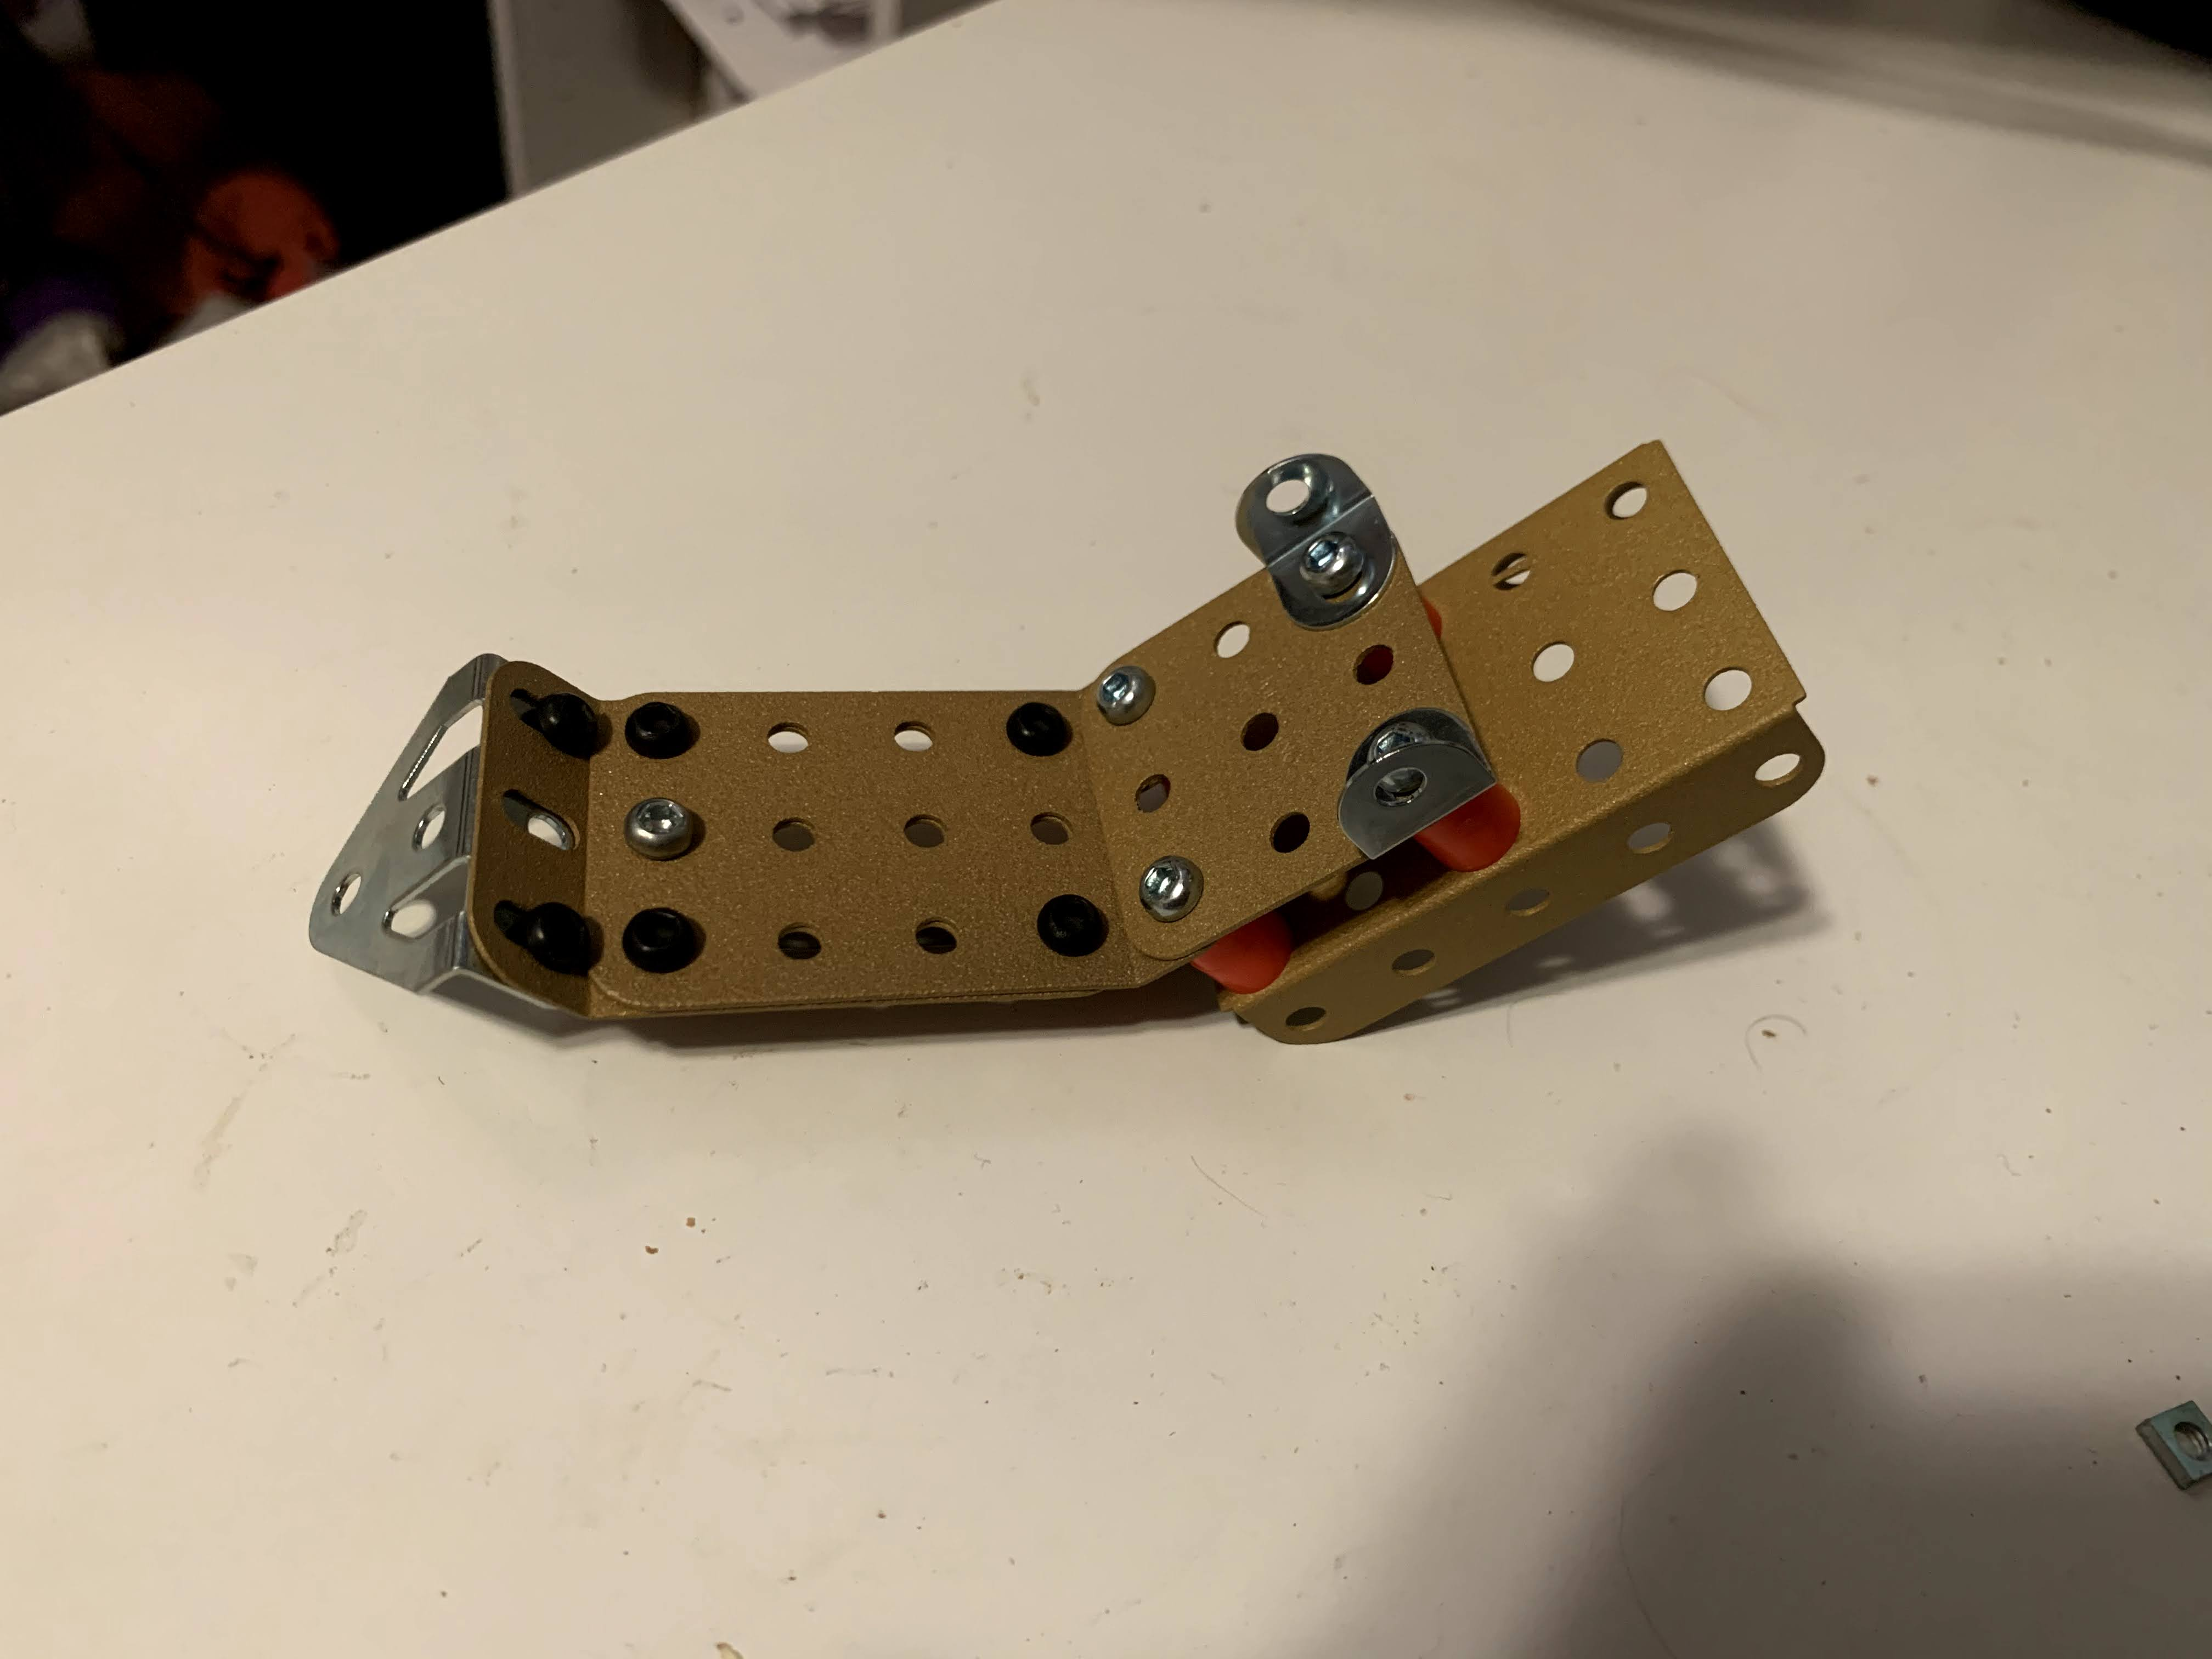
\includegraphics[width=5cm]{figures/erector/sub1.jpg}
    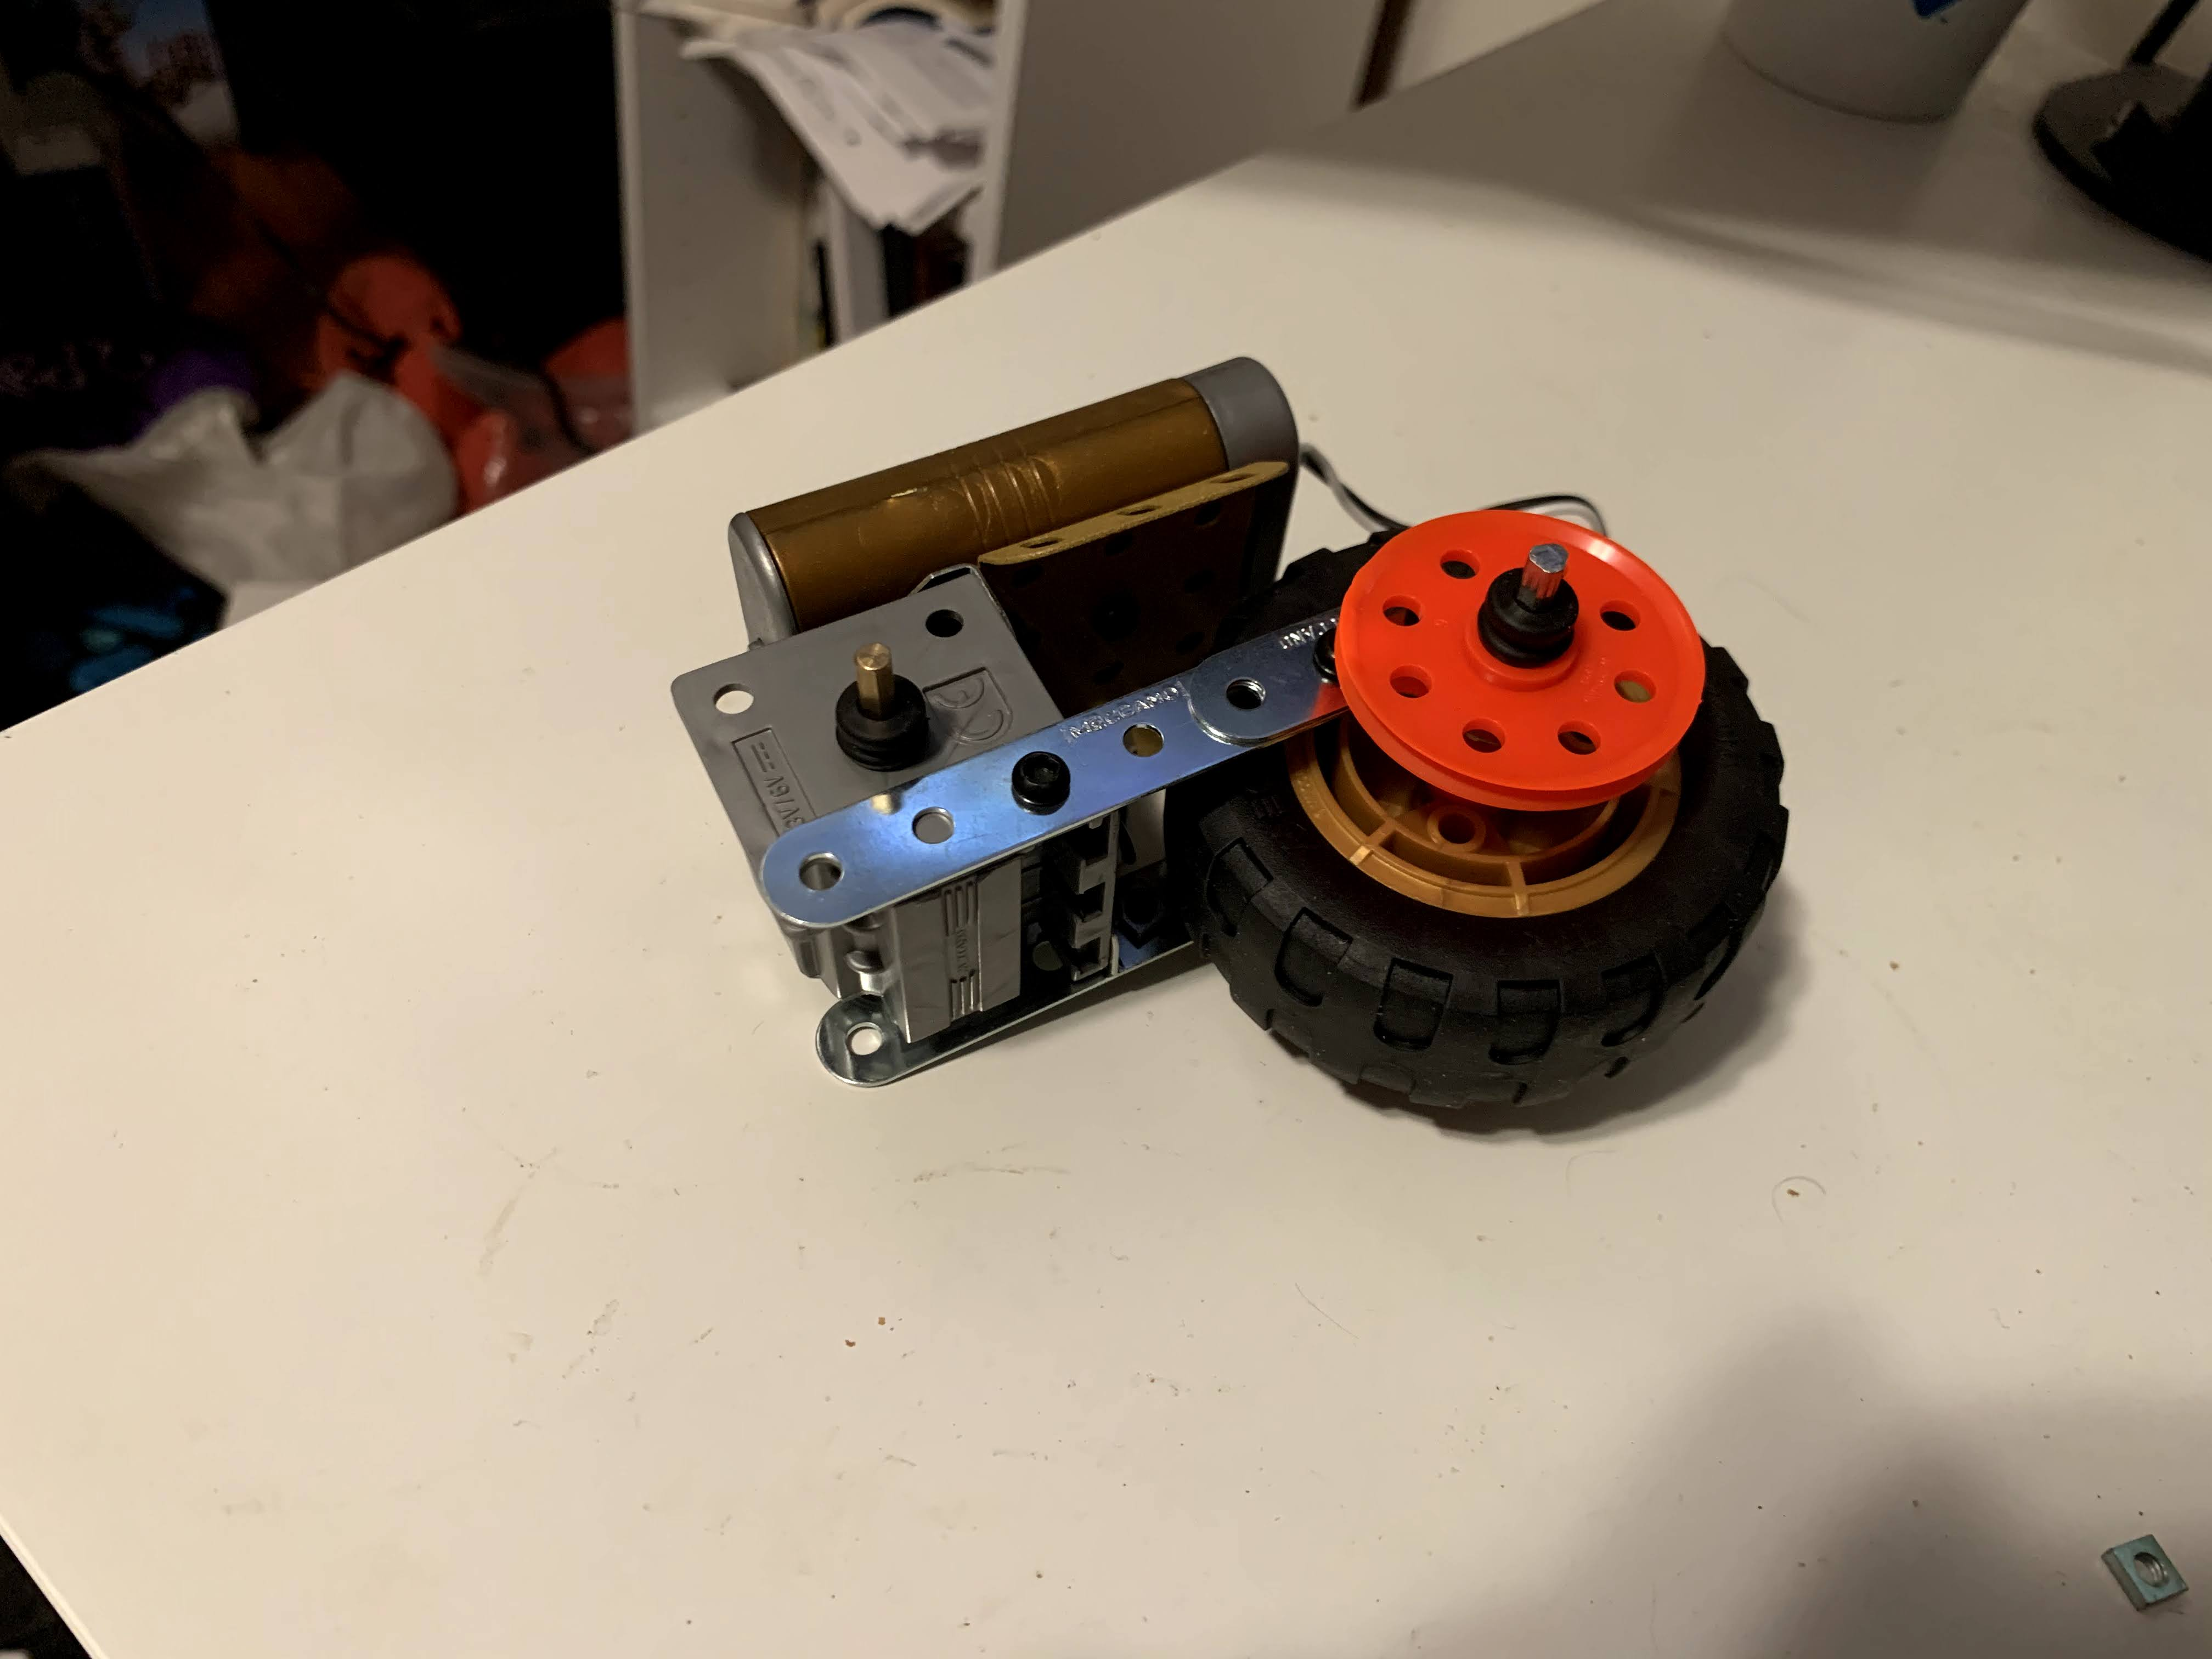
\includegraphics[width=5cm]{figures/erector/sub2.jpg}
    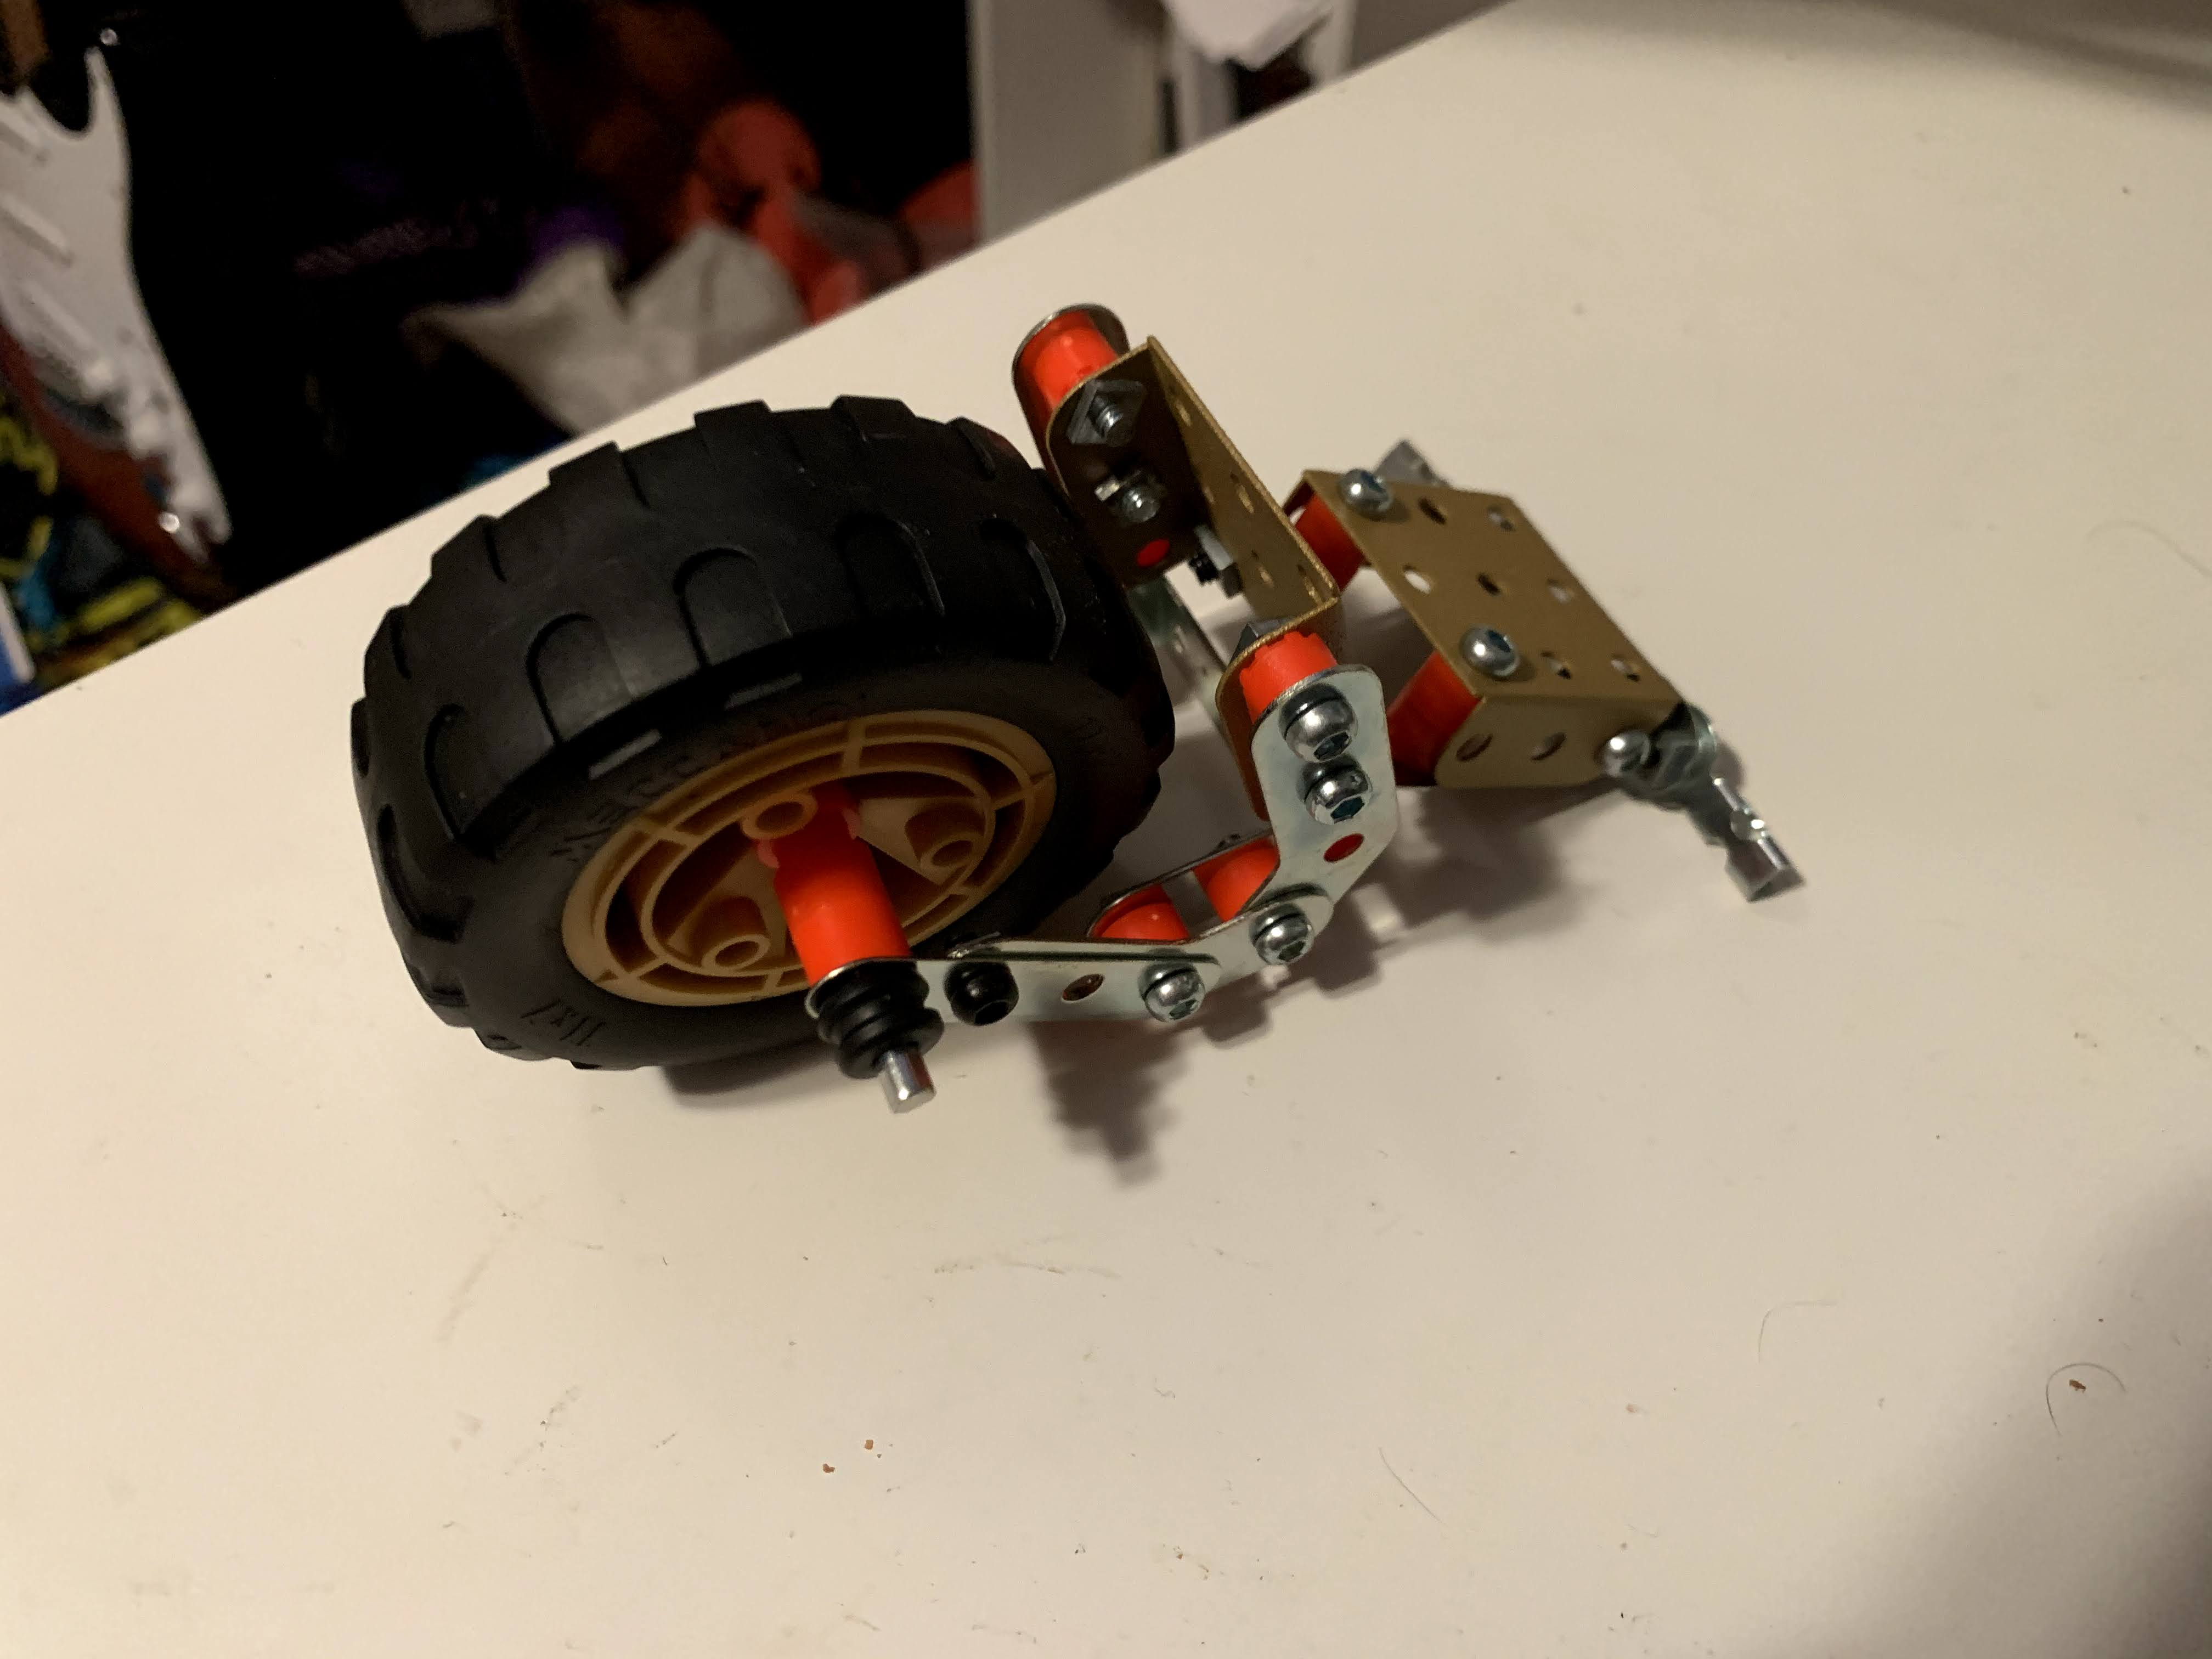
\includegraphics[width=5cm]{figures/erector/sub3.jpg}
    \caption{Sub-assemblies}
  \end{subfigure}
  \caption{A model motorcycle from a Meccano Erector kit
  }\label{fig:erector}
\end{figure}

\subsection{Implementation}

Our applications accomplish hierarchical decomposition by processing camera
images using a two stage process inspired by \citet{gebru2017finegrained}.
The first stage involves finding the region of the
image that contains the subassembly that a user is working on, using Faster
R-CNN~\cite{frcnn}.
Next, the image is cropped around this region, and the cropped region is
classified using Fast MPN-COV~\cite{Li_2018_CVPR}.
There is one Fast MPN-COV per subassembly.
The Fast MPN-COV model has one label for each step of the task that is part of
this model's subassembly.
The classification result therefore indicates the step of the task that is shown
in an image.
The application considers a step to be complete when an image from the camera
feed is classified as the label corresponding to the next step.
The architecture for this application is shown in Figure~\ref{fig:arch}.

\begin{figure}
  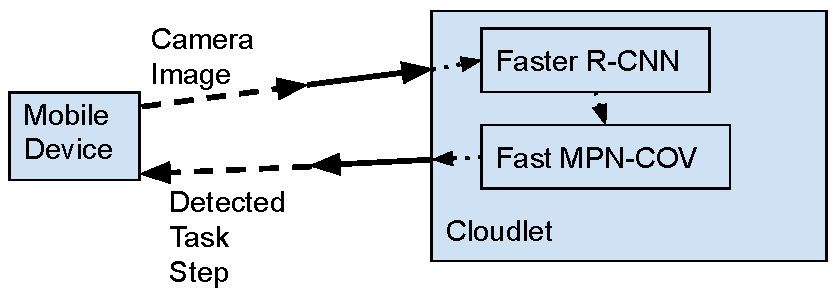
\includegraphics[width=\columnwidth]{figures/architecture.pdf}
  \caption{
    The architecture of our WCA application for the Meccano erector kit.
    The dashed lines represent a Wi-Fi connection.
    The solid lines represent a connection over Gigabit Lan.
    The dotted lines represent data transmission between components on a single
    cloudlet.
  }\label{fig:arch}
\end{figure}

A single label may correspond to multiple steps of a task.
For example, a kit might contain two identical subassemblies that get assembled
on their own, before being connected to the rest of the kit.
The steps required to assemble both of these subassemblies will be identical.
The subassemblies do not get connected to the rest of the kit until after they
have been assembled, so there will not be any visible differences while the user
is assembling one or the other.
The application can therefore use the same sequence of outputs from a computer
vision model for both subassemblies.
However, two consecutive steps cannot share the same label.
The application considers a step to be completed when images are classified with
the label corresponding to the next step.
If the next step had the same label, the application would think that the user
completed a step immediately after the step was started.
This issue is illustrated in Figure~\ref{fig:consec_step}.

\begin{figure}
  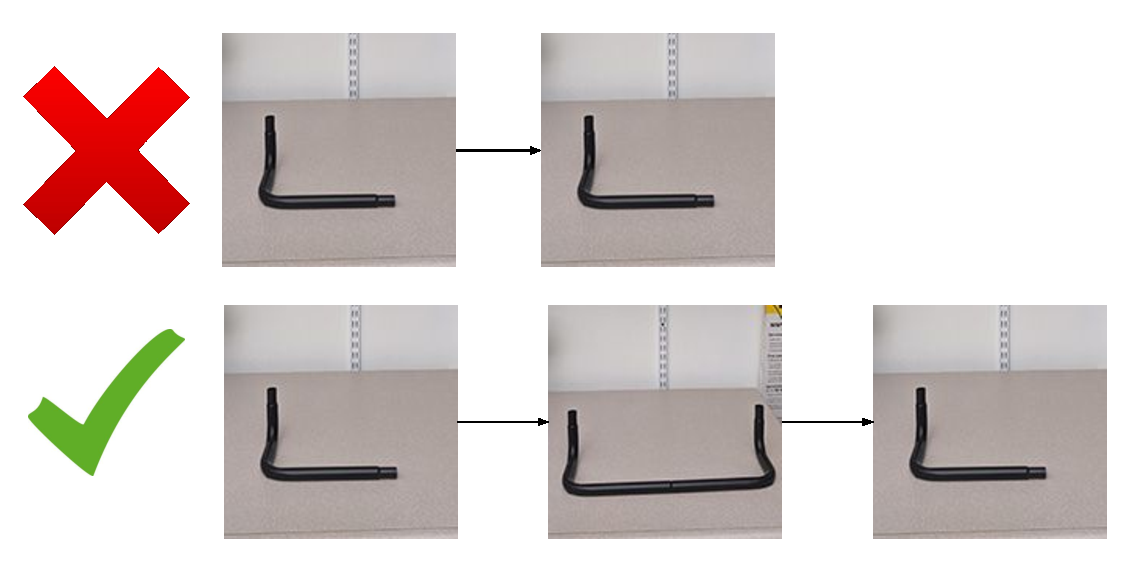
\includegraphics[width=\columnwidth]{figures/consec_step.pdf}
  \caption{
    The sequence of steps depicted in the top row cannot be supported by our
    techniques because the two consecutive steps are identical.
    The sequence of steps depicted in the bottom row is acceptable because the
    identical steps are not consecutive.
  }\label{fig:consec_step}
\end{figure}

\subsubsection{Training}

We performed transfer learning from pre-trained models, rather than training
models from scratch.
Our Fast MPN-COV models were pre-trained on ImageNet 2012~\cite{ILSVRC15} and
our Faster R-CNN models were pre-trained on COCO 2017~\cite{coco}.
We used a PyTorch~\cite{pytorch} implementation of Fast MPN-COV and a
TensorFlow~\cite{tensorflow2015-whitepaper} implementation of Faster R-CNN.

\subsubsection{Error Correction}

Developers can train fine-grained classifiers to recognize specific mistakes
that a user of a WCA application might make when trying to complete a task.
An error state requires training data, the same way other steps of the task do.
When a frame gets classified as depicting an error state, the user is given
instructions about how to correct this.
Chapter~\ref{chap:escalation} provides further discussion about handling errors
with WCA applications.

\subsubsection{Development Tools}

We expanded the Ajalon tools~\cite{pham2021ajalon} to support hierarchical
decomposition.
Ajalon previously only supported a single object detector, which was sufficient
for toy examples such as the sandwich described in~\cite{chen2017}.
However, more complex assembly task require the use of multiple object detectors
and multiple fine-grained image classifiers.
Our improvements to Ajalon allow developers to have the application use
different computer vision models as a user progresses through a task.
This results in a single application that will automatically start
giving users instructions for the next sub-assembly after they have completed
the previous one.

\section{Our Applications}

To validate our approach, We developed WCA applications for three real assembly
tasks.
We trained models for these applications using real videos that were recorded
using a smartphone.
The videos were manually annotated with bounding boxes using CVAT.
We cleaned up our dataset by computing the perceptual hash values of every
image.
For all sets of images with identical perceptual hash values, we removed all but
one of the images.
This resulted in a set of images that all had unique perceptual hash values.

We have posted\footnote{\url{https://rogeriyengar.com/thesis}} all of the
artifacts required to run these applications, along with videos showing them
being used.

\subsection{Stirling Engine}\label{sec:stirling}

This WCA application guides users through disassembling a
Stirling engine.
This task requires 22 steps. All of the parts are made out of
metal, with the exception of one ring that is made out of silicone. Some steps
just require removing a single screw, and the engine looks very similar before
and after these steps have been completed.
We split the task into four subassemblies, which are shown in
Figure~\ref{fig:stirling_subs}.

\begin{figure}
  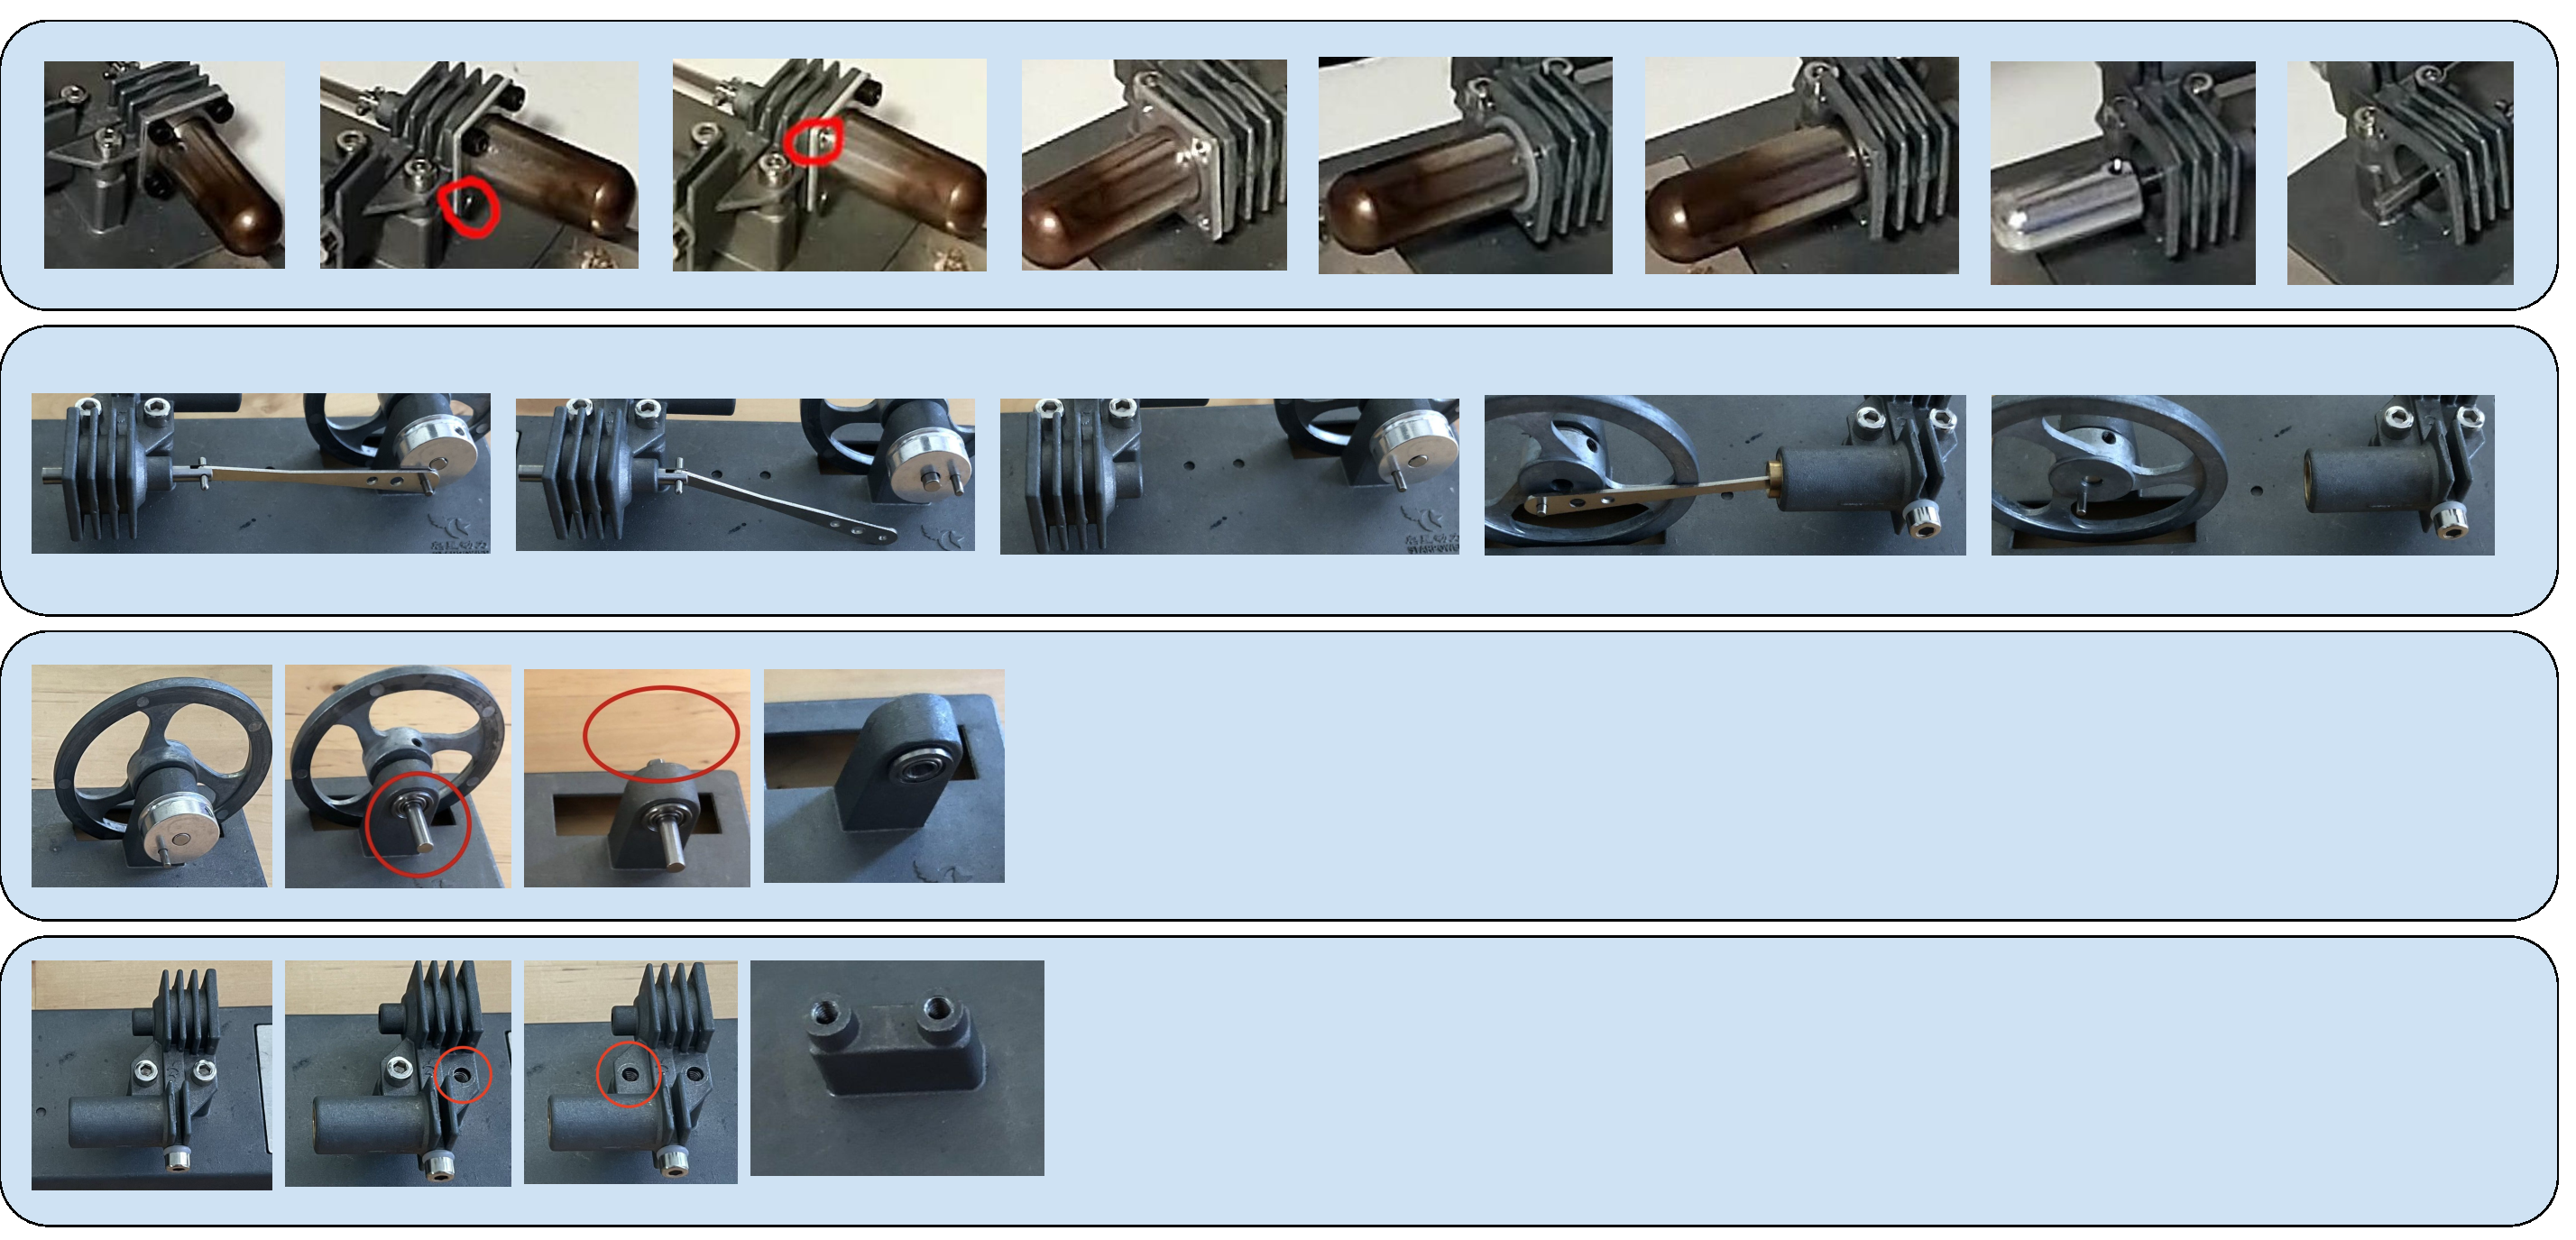
\includegraphics[width=\columnwidth]{figures/stirling_subassemblies.pdf}
  \caption{
    The steps detected by our Stirling Engine WCA application.
    The blue rectangles represent subassemblies.
    Each subassembly corresponds to a different Fast MPN-COV model.
  }\label{fig:stirling_subs}
\end{figure}

Several steps of the task involved removing screws from the engine.
The labels for these steps indicated the number of screws visible in the frame,
rather than being unique to the specific step of the task.
For example, in Figure~\ref{fig:stirling_steps}, the first and third steps
were both given the label ``2 Black Screws.''
The training script for Fast MPN-COV randomly flips images
horizontally, so we did not want the label to depend on the orientation of
objects.
The initial steps for this task all require removing screws or flipping the
engine to show screws that were previously occluded.
Therefore, every step changes the number of screws that are visible.

\begin{figure}
  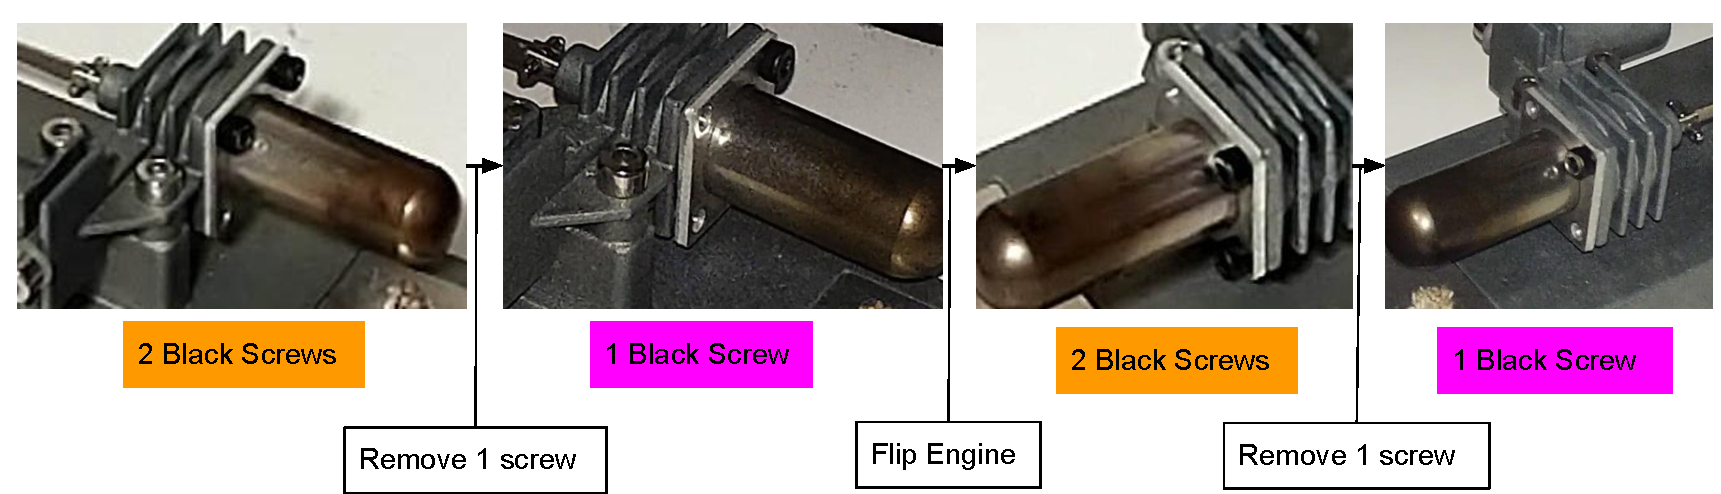
\includegraphics[width=\columnwidth]{figures/stirling_steps.pdf}
  \caption{Four states from our WCA application for a Stirling engine. The
    steps look visually similar aside from the number of screws that are
    visible. The text in colored boxes are the labels that our image classifier
    was trained on.
    Note that some different steps were given the same label, but consecutive
    steps must have different labels.
    The text in the white boxes describes the actions users take to complete a
    step.
  }\label{fig:stirling_steps}
\end{figure}

We found that illuminating the engine with a table lamp increased the accuracy
of the application beyond what we could achieve with overhead room lighting.
We lit the object the same way when capturing training data and using the
application.

\subsection{Ikea Cart}

Our next application provides guidance for users assembling an Ikea Raskog
utility cart.
The task requires twenty steps to complete successfully.
However, the cart has two pairs of identical components that must be
assembled the same way.
Therefore, four of the steps are repeats of earlier steps.
The application uses the same label in cases where steps are identical.
Thus there were 16 labels, that each corresponded to the 16 unique steps.
In addition, we developed the application to detect one error state, so there
were 17 possible labels that our models could output.
We split the task into three subassemblies, which are shown in
Figure~\ref{fig:ikea_cart}.

The repeated steps are repeated in pairs. For example, step 1 is performed,
followed by step 2.
Then both are repeated.
Repeating steps in pairs avoids the situation where two consecutive steps
correspond to the same label from the classifier.

\begin{figure}
  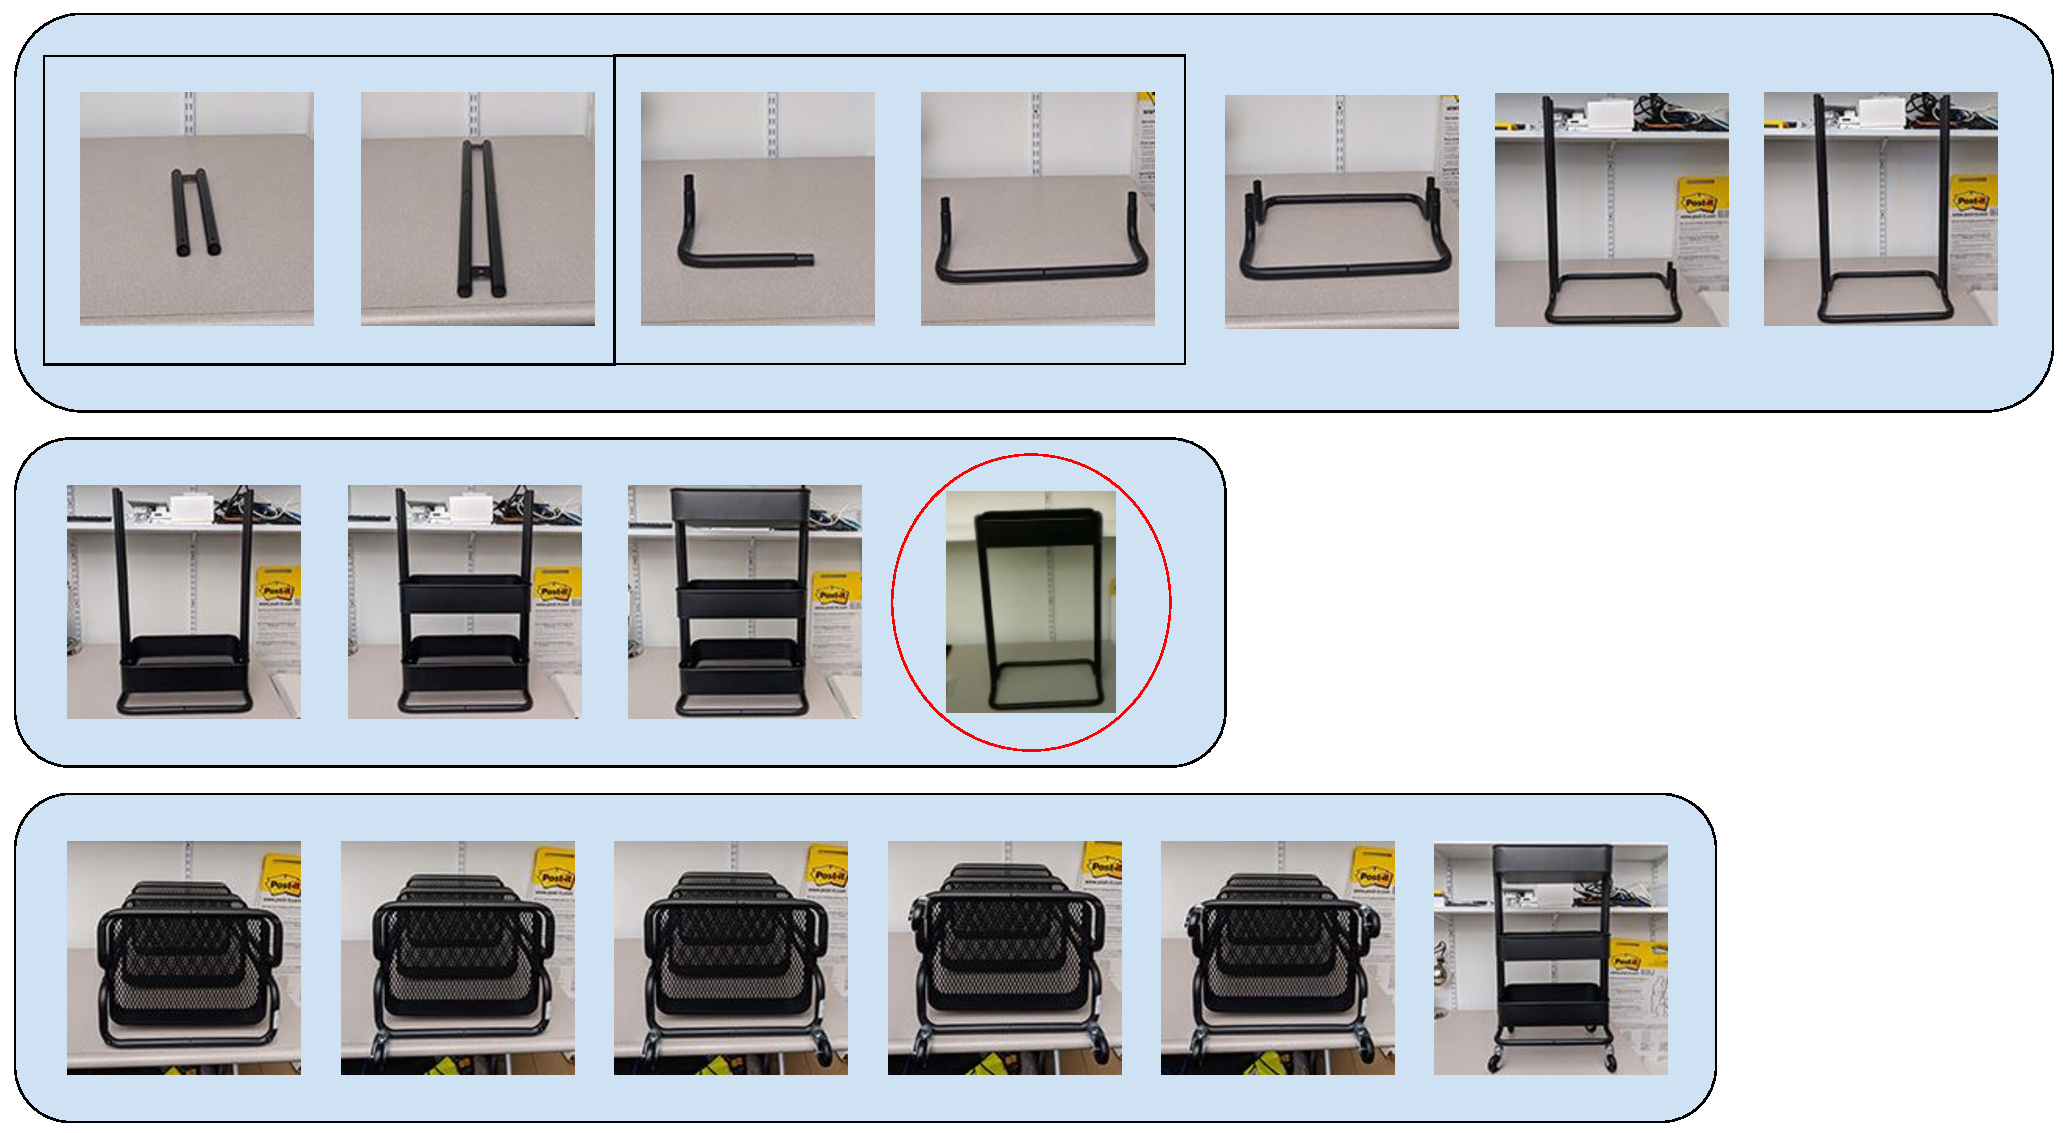
\includegraphics[width=\columnwidth]{figures/ikea_subassemblies.pdf}
  \caption{
    The steps detected by our Ikea WCA application.
    The blue rectangles with rounded corners represent subassemblies.
    The steps in the rectangles without rounded corners are repeated.
    The error state appears in the red circle.
  }\label{fig:ikea_cart}
\end{figure}

\subsection{Toy Car}

The last application guides users through assembling a model car.
This task requires 28 steps, which we split into 6 subassemblies.
These steps and subassemblies are shown in Figure~\ref{fig:toy_car}.
The computer vision models output a unique label for each step of the task.

\begin{figure}
  \includegraphics[width=\columnwidth]{figures/toycar_subassemblies.pdf}
  \caption{
    The steps detected by our Toy Car WCA application.
    The blue rectangles represent subassemblies.
  }\label{fig:toy_car}
\end{figure}

\section{Implementation Details}

We captured images at 1920x1080 pixels, and transmitted these to the cloudlet at
their full resolution.
This is the highest resolution that Android CameraX's ImageAnalysis use case
supports.
After processing the images with Faster R-CNN, the application crops them around
the region that likely contains the object.
The cropped image is resized to 448x448 pixels and then classified by Fast
MPN-COV.
By starting with a large initial image, we ensured that the cropped image would
be at least 448x448 pixels.

\subsection{Realtime Data}

The code for many computer vision models are written to run inference on batches
of images that are stored on disk. The torchvision package contains functions
for loading images from disk, in batches. Using these models in WCA applications
requires modifying the code to run the models on images being transmitted over
the network, one by one. The input batch size must be set to 1, because anything
larger would require building up a queue of images that would be run through the
model together as a single input. A larger batch size would improve the
frame rate for inference, but hurt the latency.

Live data must be as similar as possible to the data that the models are trained
on. For example, converting a
JPEG image to raw pixel values using OpenCV will result in slightly different
values than using Pillow will. We observed that our Fast MPN-COV model performed
significantly better with images opened using Pillow than with images opened
using OpenCV. The training images were opened using Pillow, but we did not
expect opening JPEGs with OpenCV and Pillow to result in different color values.

Processing images while a user is in the middle of a step wastes bandwidth and
computing resources on cloudlets.
In addition, it might lead to an application mistakenly
believing that a step has been completed before it actually has been.
We experimented with a filter that requires a set of consecutive frames to have
identical perceptual hash values.
This essentially means that a certain number of images in a row all had to look
the same.
This technique worked well for WCA applications running on a smartphone mounted
to a tripod.
But it did not work well for WCA applications running on a Google Glass, due to
the motion of the user's head.
Instead, we required a sequence of sequential images to be assigned the same
label by the classifier.
This helped avoid cases where the application mistakenly believed a step had
been completed while a user was still in the middle of it.
But it did not save computing resources on the cloudlet, because every frame had
to be processed.

\chapter{Synthetic Training Images}\label{chap:synthetic}

Training the DNNs that are used by WCA applications for physical assembly tasks
requires thousands of labeled images.
Capturing and labeling these images requires substantial effort.
Bounding boxes must be drawn around the region of each image that
contains the object being assembled.  The bounding box must then be
labeled with the step of the assembly process that is depicted in the
image.  Collecting and labeling a training set of images is a major
barrier to entry for anyone who wants to develop a WCA application for
a new task.
For example, this effort took over 50 person hours for the Ikea Cart application
described in Section~\ref{sec:ikea_cart}.
This task had 17 different states.
This time-consuming and labor-intensive
aspect of WCA is the biggest bottleneck to its widespread adoption.

Previous papers have proposed the use of synthetically generated
images for training sets.  In this approach, pre-labeling is done by
construction~\cite{synthetic_data, DBLP:journals/corr/abs-1809-10790,
  photo2, real_background1, real_background2, real_background3,
  dwibedi}.  Since programs that generate synthetic images have
information about the objects that are visible and their locations,
there is no need for manual input of this information.  In addition,
synthetic images of objects can easily be rendered in a wide variety
of different lighting conditions and environments.  In contrast,
capturing real images of objects in a variety of conditions requires
the images of the object to be captured in every such environment.
Overall, the use of synthetic data may save considerable manual
effort.

This chapter presents our experience training DNNs for WCA applications for
three assembly tasks, using synthetic training images.

\begin{figure}
  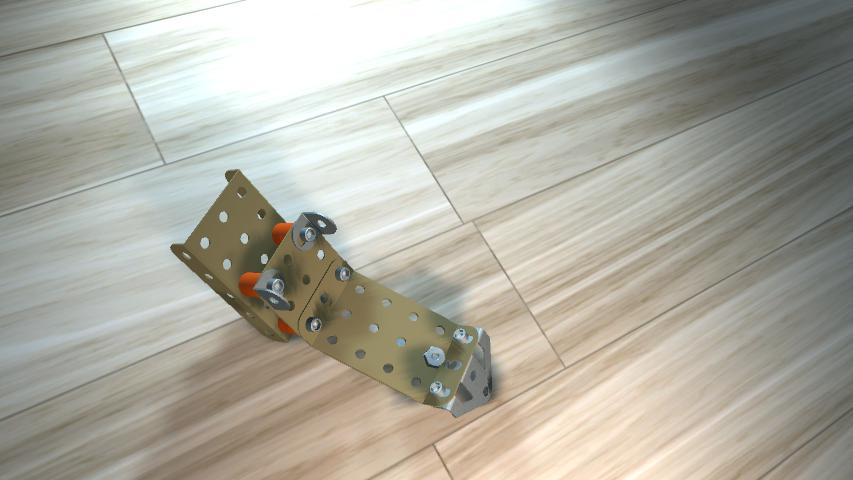
\includegraphics[width=0.5\columnwidth]{figures/synthetic/floor1.jpg}
  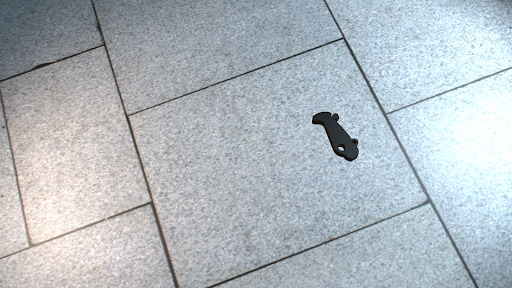
\includegraphics[width=0.5\columnwidth]{figures/synthetic/plane_train2.png}
  \caption{
    Examples of synthetically generated images
  }\label{fig:synthetic_examples}
\end{figure}

\section{Meccano Erector Kit}

In this section, we ask how well synthetic images work for creating a WCA
application for assembling a Meccano Erector Kit.
We use the following procedure to answer this
question.  We first generate a set of synthetic (pre-labeled) images
using the Unity Perception package~\cite{unity}.
Unity is a video game engine that includes 3D graphics rendering capabilities
and CAD tools.
The Perception package was created by Unity to enable the creation of object
detectors from CAD models instead of real images that had to be labeled with
bounding boxes.
This package can create thousands of images, and it will render the subassembly
in a different location in each one.
It outputs a label file with each image, that contains the coordinates that the
subassembly in that image was rendered at.
This eliminates the need to manually label images with bounding boxes.

After generating the synthetic images with Unity, we train
computer vision models on this data.  Next, we  collect and manually
label a set of real images for the same task, and then train computer
vision models on this data.  Finally, we compare the accuracy of these
two families of models on a held-out test set of real images.  Our
results show that models created with a training set size of 75,000
synthetic images perform slightly better than models created with
roughly 15,000 real images.
However, this ordering is reversed when fewer synthetic images are used for
training.

The Meccano Kit assembles into a model bike.
The fully assembled model is depicted in Figure~\ref{fig:full_bike}.
It is made from over 50 parts.
However, this work will only separate the bike into three subassemblies.
The fine-grained classifiers we trained for this kit had 5 output labels.
Three of the labels were for the individual subassemblies, and the remaining two
were for the steps required to put the subassemblies together.

\begin{figure}
  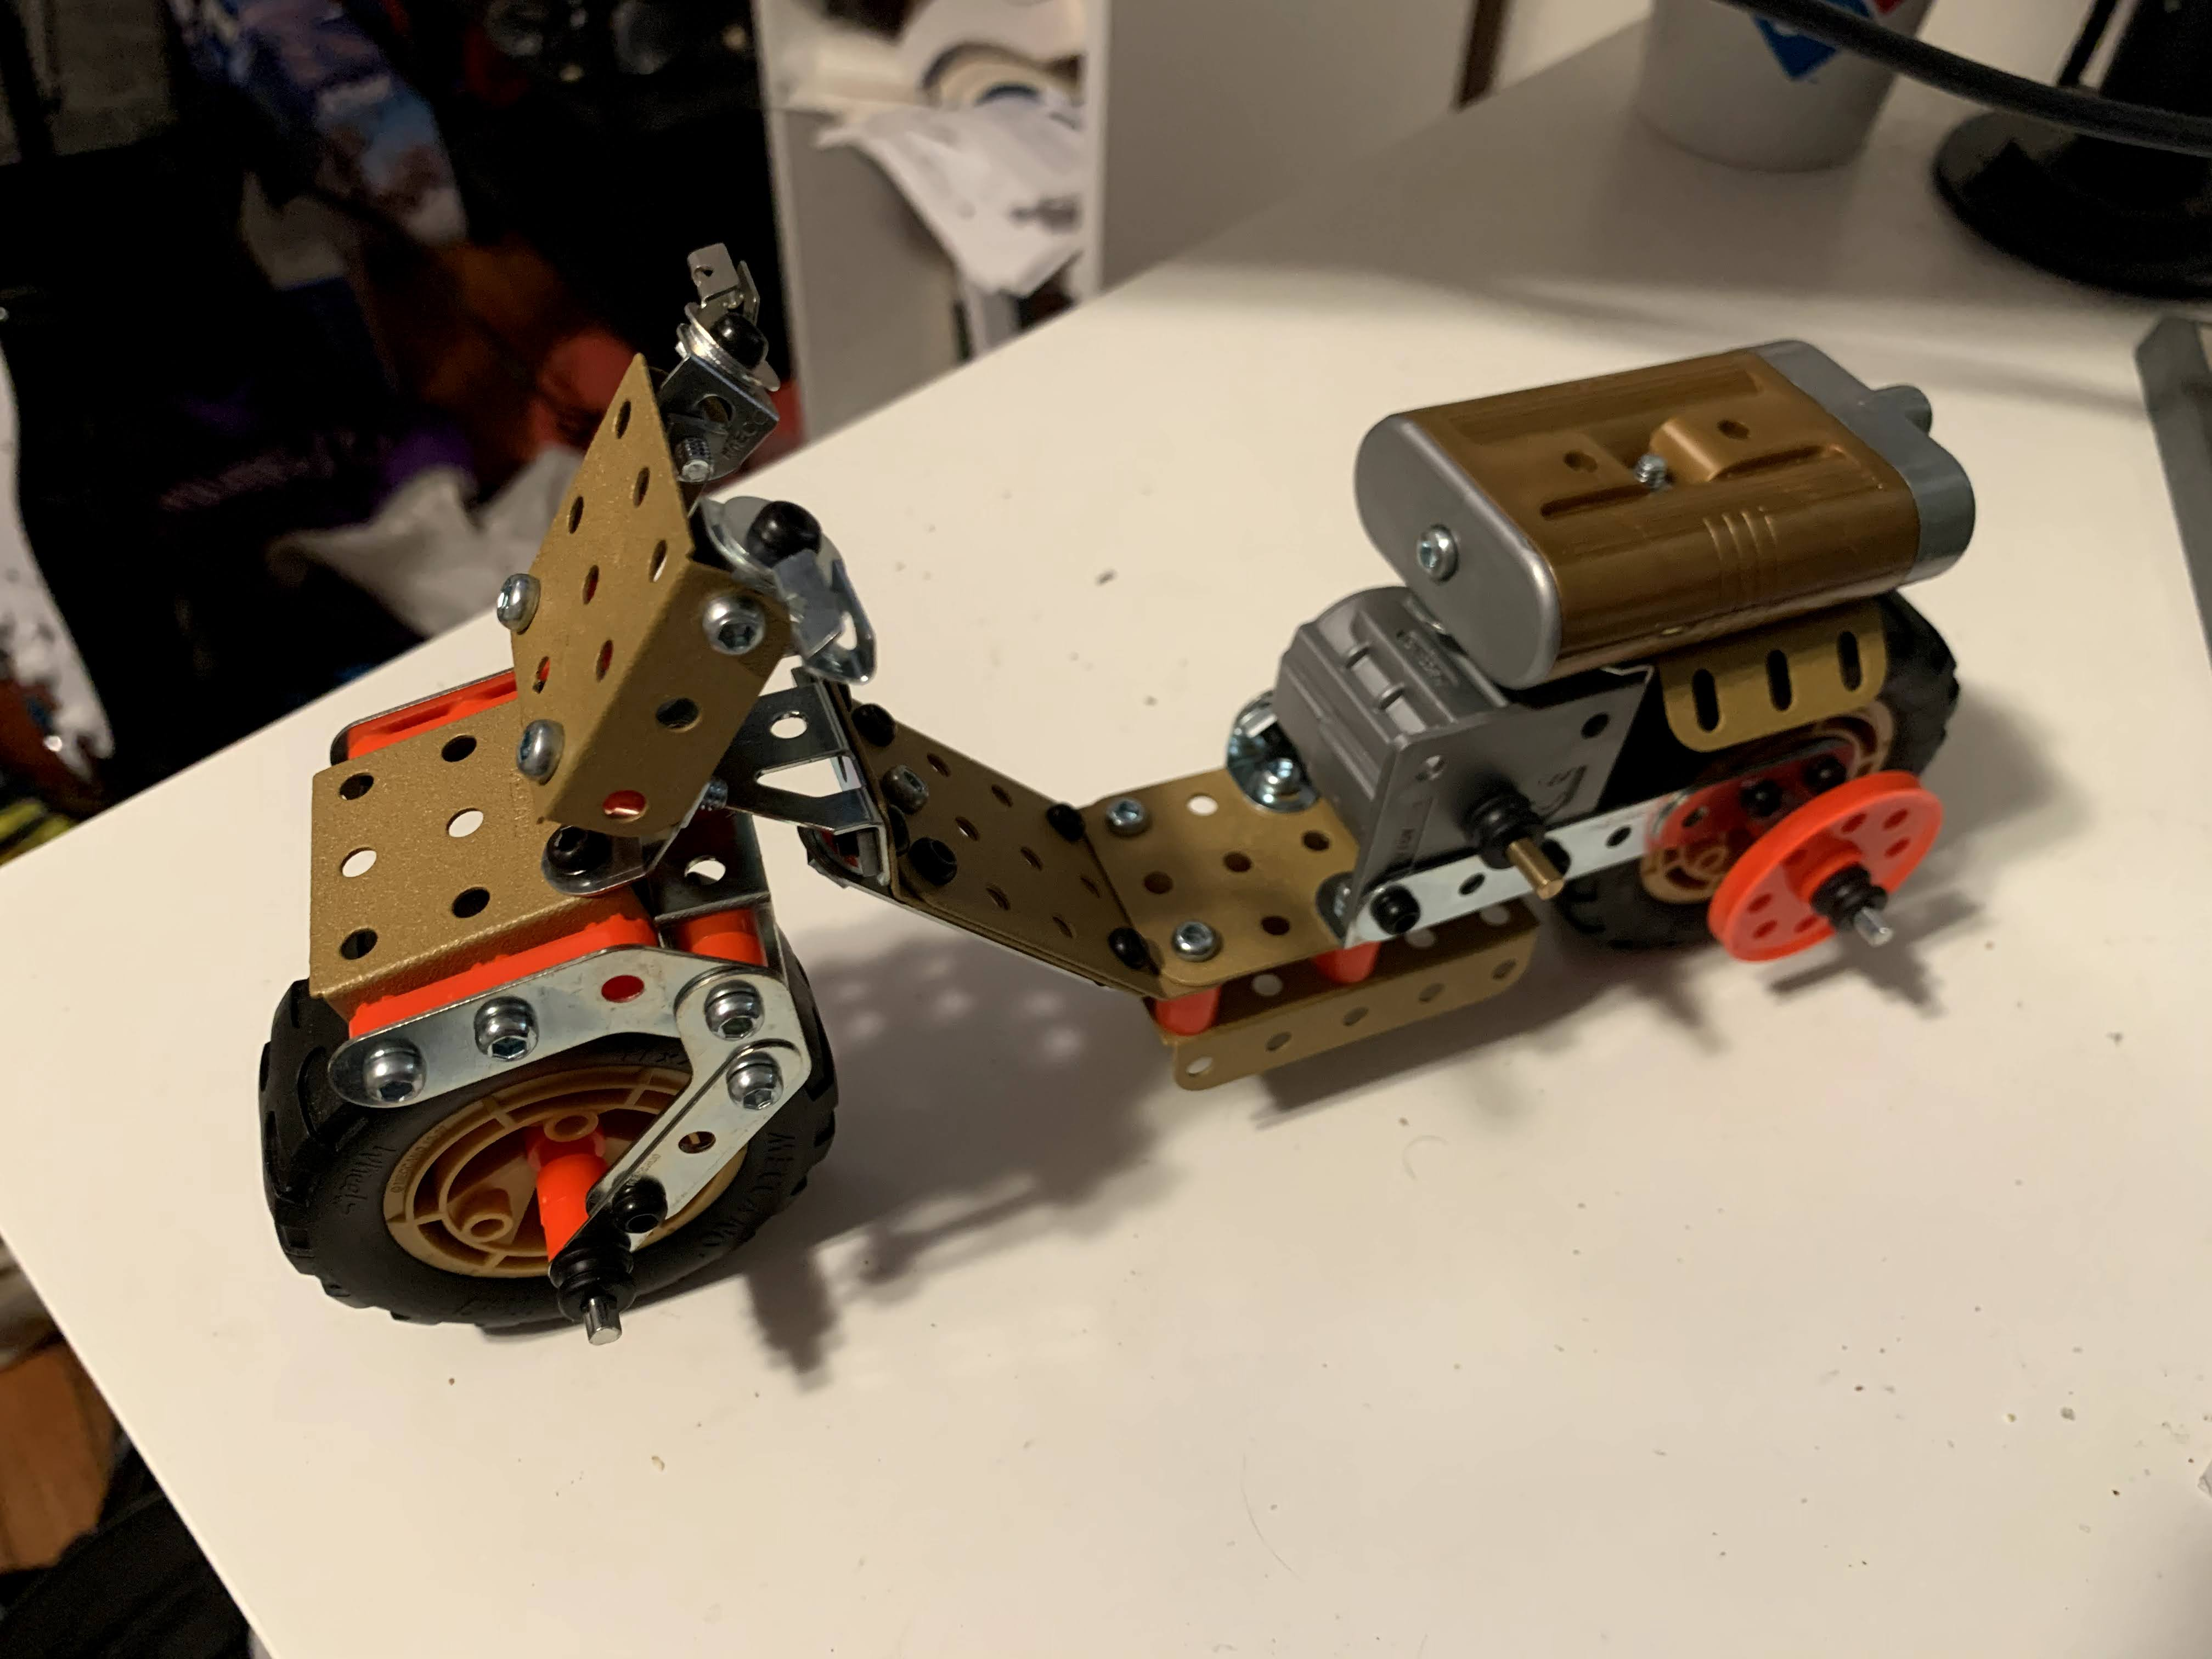
\includegraphics[width=\columnwidth]{figures/synthetic/full_bike.jpg}
  \caption{
    The fully assembled model bike
  }\label{fig:full_bike}
\end{figure}

\subsection{Generating Data}

We found a computer-aided design (CAD) model for the Meccano kit on the
community website
GrabCAD\footnote{\url{https://grabcad.com/library/meccano-9550-002-1}}.
This CAD model appears to have been created to replicate the physical Meccano
pieces, rather than being the same model that was used to manufacture the
pieces.
In particular, we noticed a number of differences between the CAD model and the
actual Meccano parts.
We selected textures for each part of the model, trying to match the
appearance of the physical object as closely as possible.
We generated synthetic images using the Unity Perception Package~\cite{unity}.
The default setup for this package fills the background of the images that are
generated with objects that the network should learn to ignore.
Figure~\ref{fig:perception_default} shows an image generated using this default
setup.

\begin{figure}
  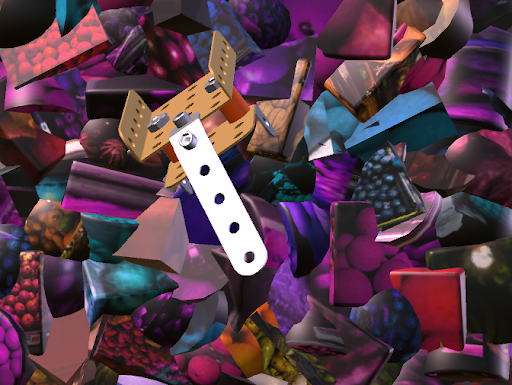
\includegraphics[width=\columnwidth]{figures/synthetic/perception_default.png}
  \begin{captiontext}
    The background is filled with distractor objects that the network should
    learn not to identify.
  \end{captiontext}
  \caption{
    A synthetic image showing part of the bike model
  }\label{fig:perception_default}
\end{figure}

The Unity Perception Package allowed us to make some of the individual parts of
the CAD model invisible.
This enabled us to generate synthetic images for each step of the task.
For a given step, we specified the parts of the subassembly that were visible.
We were then able to generate thousands of synthetic images for this step.
The perception package generated a label file for each synthetic image, that
specified the coordinates of a bounding box around the subassembly and a label
name corresponding to the step of the task that was shown in the image.

We trained a Faster R-CNN object detector using this data.
The Unity package creates a file with bounding box and label information, and
we converted this to the format used by the TensorFlow Object Detection API.
The perception package drew bounding boxes tightly around the objects.
We added padding to these bounding boxes, to make them more like our hand-drawn
labels (which also had some padding).
Figure~\ref{fig:padding} shows bounding boxes with and without padding.
Training the object detector on images with padding resulted in the object
detector returning bounding boxes with some padding.
This resulted in higher intersection over union scores when evaluating our
object detectors on test data with hand-drawn labels.

\begin{figure}
  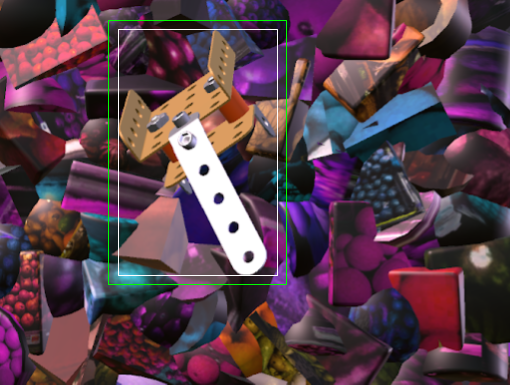
\includegraphics[width=\columnwidth]{figures/synthetic/padding.png}
  \begin{captiontext}
    The white bounding box has no padding.
    The Unity perception package uses bounding boxes without padding.
    The green bounding box has padding.
    Our dataset uses bounding boxes with padding.
  \end{captiontext}
  \caption{
    Bounding boxes with and without padding
  }\label{fig:padding}
\end{figure}

Unfortunately the training process for this model did not converge.
\hl{This might have occurred because it is difficult to differentiate the
  object we want to detect from the brightly colored distractor objects in the
  background.}
We attempted to fix this issue by removing the background objects from the
image, and then we tried to make the objects look like they were sitting on a
wooden floor.
We accomplished this by placing the object at the bottom of the 3D scene in
Unity and texturing the floor of the scene with an image of wood from Adobe's
collection of stock images.
Figure~\ref{fig:wood_floor} shows one of these images.
The Faster R-CNN model trained on this data converged; however, it performed
poorly.
One issue that we noticed was the object detector mistakenly detected lines
in the wood floor as being a model bike assembly.
Figure~\ref{fig:false_positive} shows an example of such an erroneous detection.

\begin{figure}
  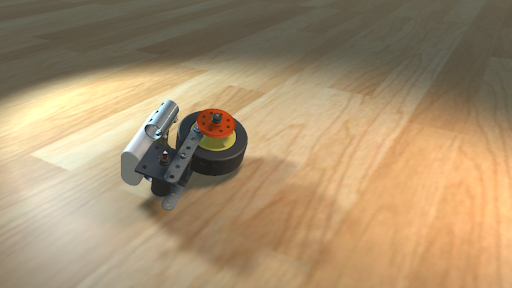
\includegraphics[width=\columnwidth]{figures/synthetic/wood_floor.png}
  \begin{captiontext}
    This image is meant to look like an object sitting on a wood floor.
  \end{captiontext}
  \caption{
    Our first attempt at making our synthetic images look more realistic
  }\label{fig:wood_floor}
\end{figure}

\begin{figure}
  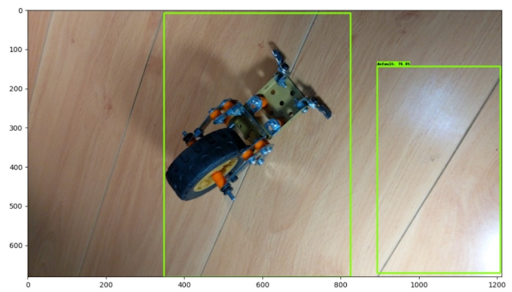
\includegraphics[width=\columnwidth]{figures/synthetic/false_positive.png}
  \begin{captiontext}
    The green bounding boxes are regions of the image in which the model
    detected an object.
  \end{captiontext}
  \caption{
    Our model incorrectly detected a line in the floor as an object of interest
  }\label{fig:false_positive}
\end{figure}

\hl{
We were able to correct this issue by using 15 additional background textures
and
randomizing the lighting in the scene and the position of the camera.
We did not conduct an experiment to determine the minimum number of background
textures that are required to achieve good performance.
}
We have posted our code\footnote{\url{https://github.com/exiaohuaz/data-gen}}.
Figure~\ref{fig:good_data} shows some examples of this data.
Figure~\ref{fig:adobe_backgrounds} shows some of the background images that we
used.

\begin{figure}
  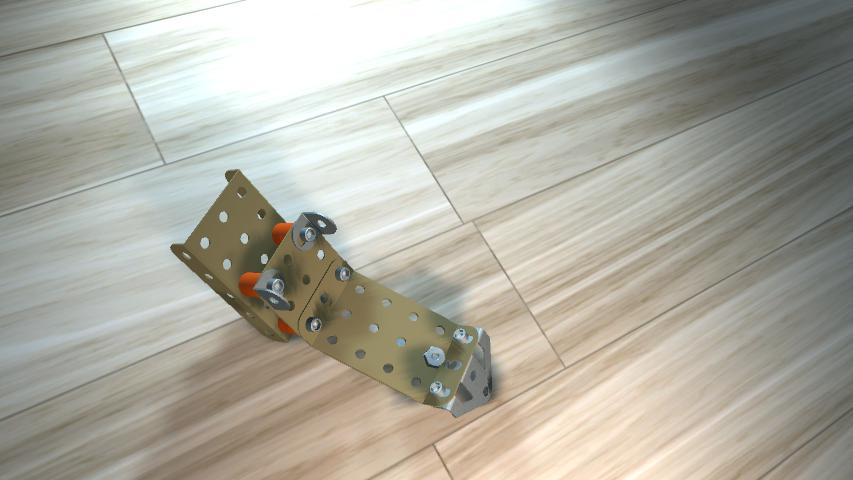
\includegraphics[width=0.5\columnwidth]{figures/synthetic/floor1.jpg}
  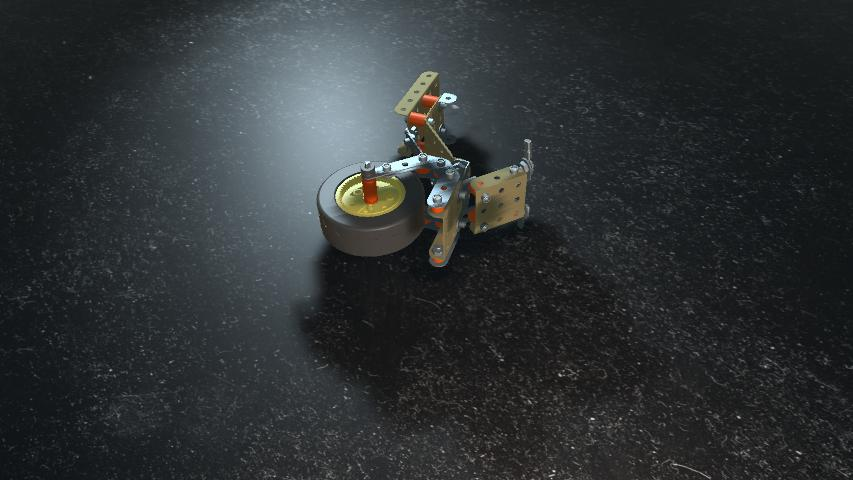
\includegraphics[width=0.5\columnwidth]{figures/synthetic/floor2.jpg}
  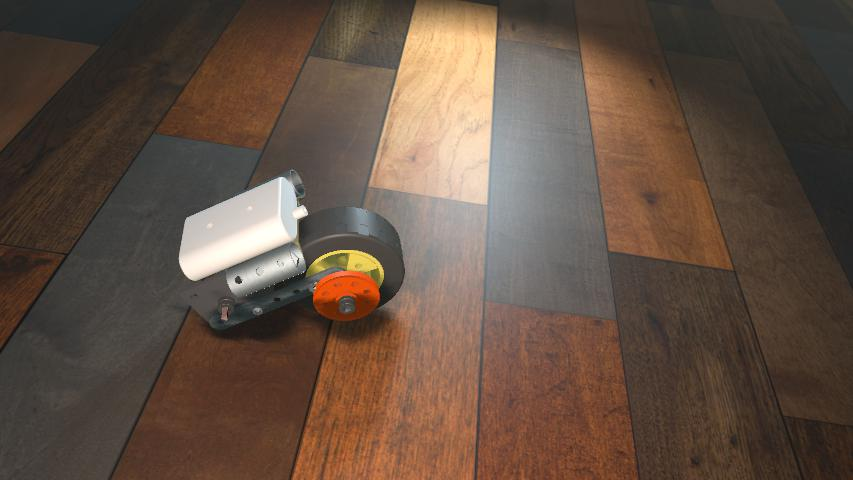
\includegraphics[width=0.5\columnwidth]{figures/synthetic/floor3.jpg}
  \begin{captiontext}
    The models trained on this data performed well.
  \end{captiontext}
  \caption{
    Synthetically generated images from our final set
  }\label{fig:good_data}
\end{figure}

\begin{figure}
  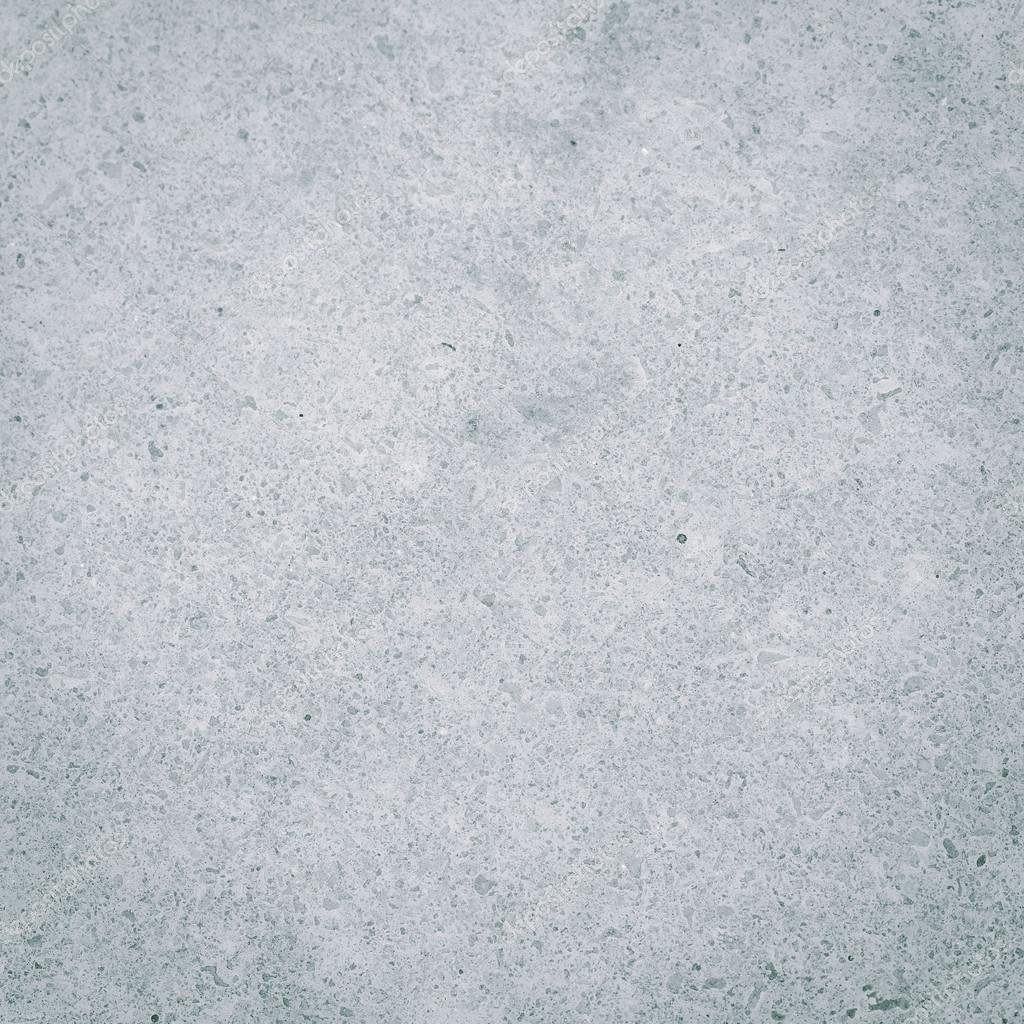
\includegraphics[width=0.33\columnwidth]{figures/adobe_stock/concrete.jpg}
  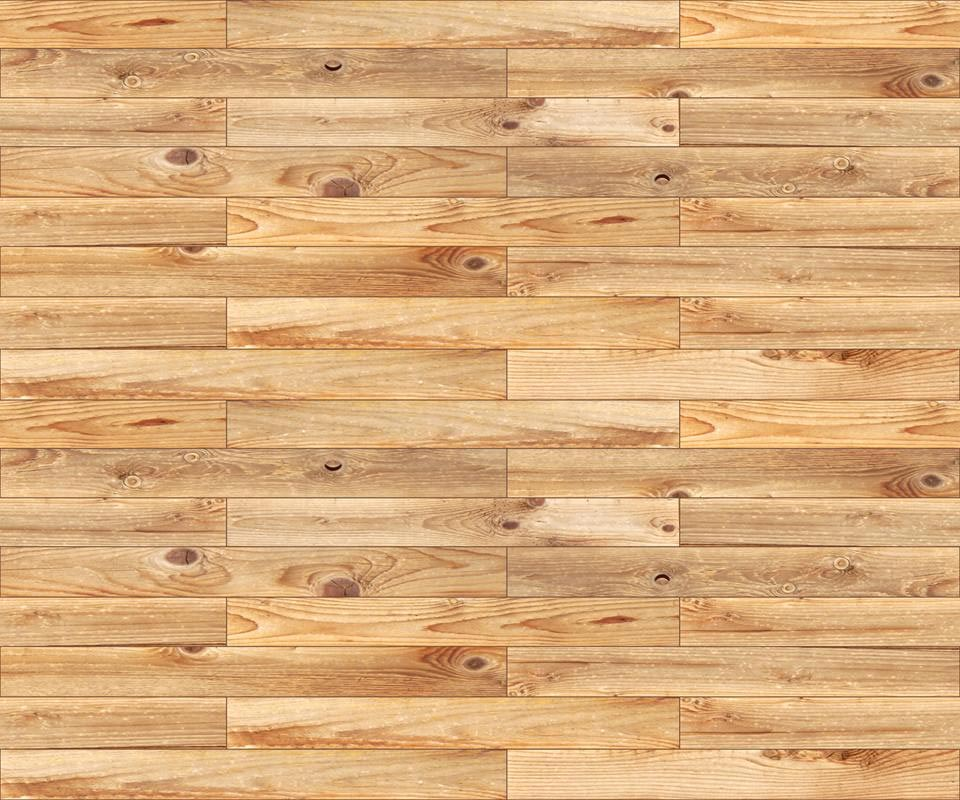
\includegraphics[width=0.33\columnwidth]{figures/adobe_stock/wood1.jpg}
  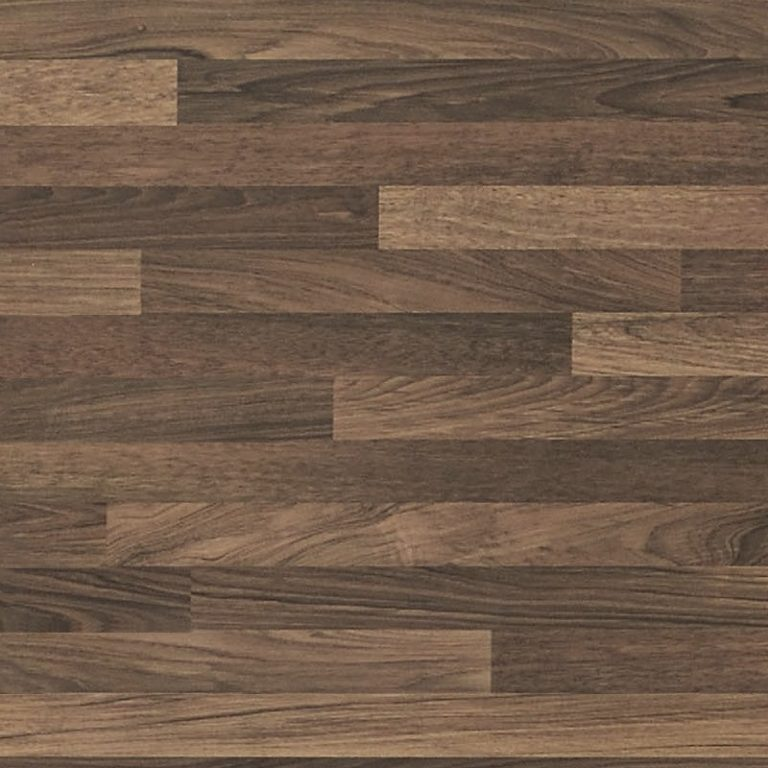
\includegraphics[width=0.33\columnwidth]{figures/adobe_stock/wood2.jpg}
  \caption{
    Examples Images from Adobe Stock that we used as background textures
  }\label{fig:adobe_backgrounds}
\end{figure}

After training the Faster R-CNN object detector to find the location of a
subassembly, we trained a Fast MPN-COV classifier to determine the step of the
task that is shown in the region found by the Faster R-CNN model.
Henceforth, we will use the term \emph{model pair} to describe a Faster R-CNN object
detector and a Fast MPN-COV classifier created using the same training set.
\hl{The two stage process was required to achieve acceptable accuracy.
  Section~{\ref{sec:single_model}} examines using a single model instead of the
  two stage process.
}

\subsection{Results}

We evaluated our model pipelines based on accuracy, which is the percentage of
images in the test set that were classified correctly.
This is equivalent to both top-1 accuracy and micro F1 score.
Classification tasks are typically evaluated using top-K accuracy, which
looks at the K labels that the model outputs as being most likely.
If any of the K labels are correct, the output is considered correct.
The value of K is varied based on what seems reasonable for the specific task.
Setting K to 5 makes sense for a dataset like Imagenet, with 1000 different
labels.
However, all of our models were trained on labels for a single subassembly.
Each subassembly was built in under 10 steps, so our models had fewer than 10
output labels.
In addition, a WCA application can only give a user one instruction at a time.
Our classifiers must reliably output the one correct label in order to be
useful.
We thus chose top-1 accuracy as our evaluation metric, rather than selecting a
larger value of K.

All of our training and testing data relates to
uncluttered environments with good lighting.
We assume that a human
using a WCA application can correct environmental issues to reduce
classification complexity.  For example, the user can increase the
amount of light shining on an assembly, or remove clutter from the
background.
Assuming near-optimal environmental conditions for a WCA assembly
task is thus reasonable.

We trained one model pair on real data that was manually labeled with
bounding boxes and class labels (15,477 images).
The remaining model pairs were trained on synthetic data sets of varying size
(12,000, 25,000, 50,000 and 75,000 images).
The labels for these images were generated by Unity.
We compared the accuracy of these model pairs.

Our test set consists of 4490 real images that are not included in any
training set.  Table~\ref{tab:meccano_accuracy} presents our results.  We
observe that the model trained on real data performs better than the
models trained on synthetic datasets with 12,000, 25,000, and 50,000
images.  However, this relationship is reversed for a model trained on
75,000 synthetic images.
Somewhere between 50,000 and 75,000 images
lies the cross-over point at which the increased number of synthetic
images more than compensates for their lower realism.
Changing the quality of the synthetic data, changing the quality of the real
data, or changing the amount of real data could change the location of the
cross-over point.

\begin{table}
\begin{tabular}{|l||l|l|}
\hline
  Dataset Type & Training Set Size & Accuracy\\
  \hline
  \hline
  Synthetic & 12,500 & 69.6\%\\
  Synthetic & 25,000 & 79\%\\
  Synthetic & 50,000 & 84.1\%\\
  Synthetic & 75,000 & 89\%\\
  \hline
  Real & 15,477 & 84.5\%\\
\hline
\end{tabular}
\begin{captiontext}
    \hl{Accuracy is the percentage of our 4490 test images that the model pairs
    classified correctly.}
  \end{captiontext}
  \caption{
    Classification results for model pairs trained on data for the Meccano kit
  }\label{tab:meccano_accuracy}
\end{table}

\section{Toy Plane}

The next kit we generated synthetic images for was a toy plane that was made up
of 3D printed plastic parts.
This kit contained six unique parts, and required four steps to assemble.
Figure~\ref{fig:assembled_plane} shows what the physical kit looks like when it
is fully assembled.
Figure~\ref{fig:plane_parts} shows the CAD models for the individual parts while
Figure~\ref{fig:plane_steps} shows the CAD models for the assembly steps.

\begin{figure}
  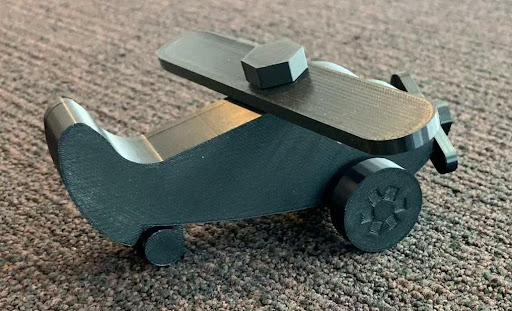
\includegraphics[width=\columnwidth]{figures/synthetic/toy_plane.jpg}
  \begin{captiontext}
    All parts are 3D printed plastic
  \end{captiontext}
  \caption{
    The fully assembled model plane kit
  }\label{fig:assembled_plane}
\end{figure}

\begin{figure}
  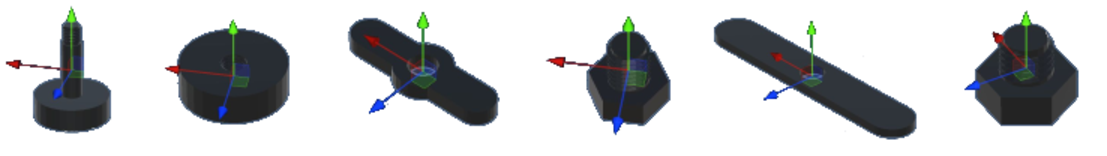
\includegraphics[width=\columnwidth]{figures/synthetic/plane_parts.pdf}
  \caption{
    CAD models for the individual model plane parts
  }\label{fig:plane_parts}
\end{figure}

\begin{figure}
  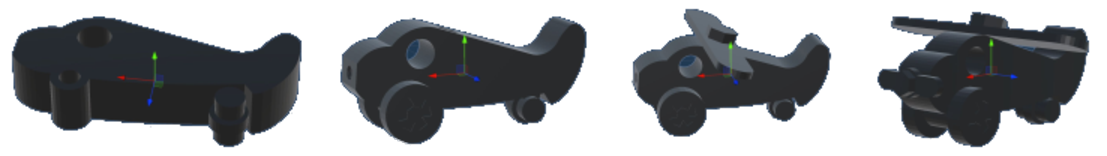
\includegraphics[width=\columnwidth]{figures/synthetic/plane_steps.pdf}
  \caption{
    CAD models for the model plane assembly steps
  }\label{fig:plane_steps}
\end{figure}

We downloaded the CAD file for this kit from the community website
Cults~\footnote{\url{https://cults3d.com/en/3d-model/game/toy-plane-assembled-by-bolts-and-nuts}},
and then 3D printed the kit using this file.
We will refer to objects generated from a CAD model that we have access to as
being ``born digitally.''

\hl{
We captured real images of the 3D printed parts using a smartphone camera,
labeled these images with CVAT~{\cite{CVAT}}, and trained a model pair on this
data.
A review of the labeling confirmed that there were no errors.
}
Next, we generated synthetic training images using the Unity Perception Package.
Figure~\ref{fig:plane_train} contains examples of these images.
Afterwards, we trained model pairs on sets of these synthetic images, with
varying sizes.

All of our model pairs for the toy plane were tested on a set of 14,996 real
images that was separate from any of the images used during training.
The results of these tests are shown in Table~\ref{tab:plane_accuracy}.
All of our model pairs that were trained on synthetic images performed better
than the model pair trained on 39,643 real images.
This was different than what we observed with the Meccano kit.
The model pair trained on 75,000 synthetic training images of the Meccano
kit outperformed the model pair trained on real images of the Meccano kit.
However, the model pair trained on real images of the Meccano kit outperformed
all of the model pairs trained on fewer than 75,000 synthetic images.
One possible reason that synthetic data was more effective for the toy plane
than the Meccano kit is that training on synthetic data might be more effective
for objects with simpler surfaces.
The toy plane is made out of simple plastic, while the Meccano kit is made out
of more complex metals.

To further investigate why all models trained on synthetic images of the toy
plane outperformed the model trained on real images, but the model trained on
real images of the Meccano kit outperformed some of the models trained on
synthetic images, new training and test sets of real images of both kits should
be collected and labeled.
The experiments should be repeated with this new data, in order to see if the
same trend still occurs.
If the relative performance of the models trained on real data still differs,
the experiment should be repeated with a different pair of kits.
As with the toy plane and Meccano kit, one kit should be made out of simple
plastic, while the other kit should be made out of complex metals.

As we observed with the Meccano kit, the accuracy of our models for the toy
plane increased with the size of the training set.
However, the increases in accuracy were less dramatic than the increases in
accuracy for the Meccano kit, because the model pair trained on the smallest
dataset achieved a high accuracy.

\begin{figure}
  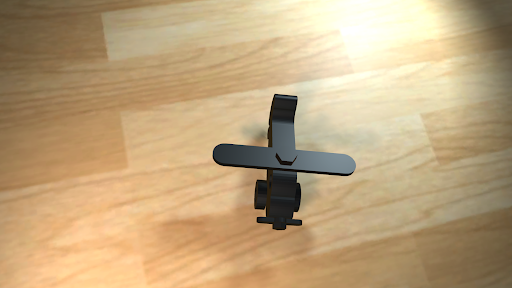
\includegraphics[width=0.5\columnwidth]{figures/synthetic/plane_train1.png}
  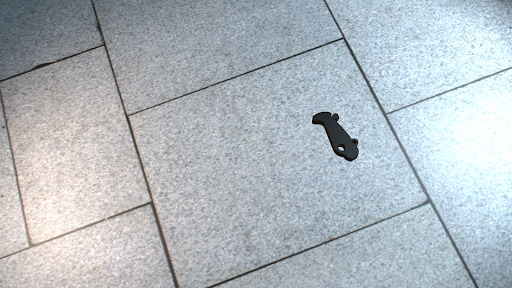
\includegraphics[width=0.5\columnwidth]{figures/synthetic/plane_train2.png}
  \caption{
    Synthetically generated training images for the toy plane kit
  }\label{fig:plane_train}
\end{figure}

\begin{table}
\begin{tabular}{|l||l|l|}
\hline
  Dataset Type & Training Set Size & Accuracy\\
  \hline
  \hline
  Synthetic & 12,500 & 87.7\%\\
  Synthetic & 25,000 & 89.3\%\\
  Synthetic & 50,000 & 90.0\%\\
  \hline
  Real & 39,643 & 76\%\\
\hline
\end{tabular}
\begin{captiontext}
    Accuracy is the percentage of our 14,996 test images that the pipeline of
    models classified correctly.
  \end{captiontext}
  \caption{
    Classification results for model pairs trained on data for the toy plane
  }\label{tab:plane_accuracy}
\end{table}

\section{Phone Sanitizer}

The final kit we generated synthetic training data for was a sanitizer for a
smartphone.
This kit contained a large metal base and several plastic parts.
Figure~\ref{fig:full_sanitizer} shows the kit fully assembled.
The kit contained four unique parts, and there were five steps required to
assemble it.
Thus there were 9 output labels from the fine-grained classifier.

\begin{figure}
  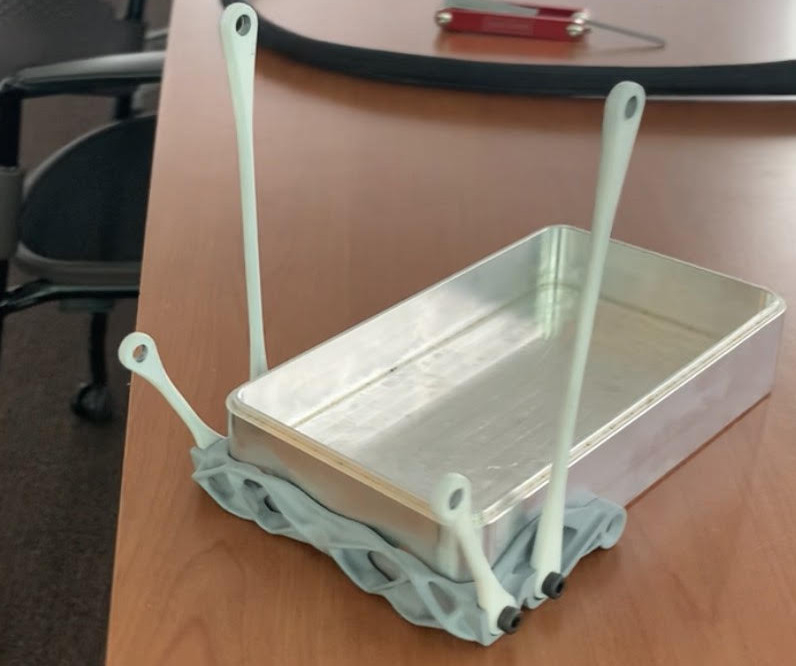
\includegraphics[width=\columnwidth]{figures/synthetic/full_sanitizer.jpg}
  \caption{
    The fully assembled Phone Sanitizer
  }\label{fig:full_sanitizer}
\end{figure}

As with the toy plane, this kit was born digitally, and we had access to the
CAD files that the parts were manufactured from.
We generated synthetic training images for the sanitizer using the Unity
Perception~\cite{unity} package and Autodesk A3D~\cite{Wang_2022_CVPR}.
Figure~\ref{fig:sanitizer_unity} shows images from the training set that was
generated using Unity while Figure~\ref{fig:sanitizer_a3d}
shows images from the training set that was generated using
A3D.
Both sets of data were used to train model pairs that were then evaluated on
60,129 real images.
As with all data that we labeled in this work, we reviewed all labeling and
confirmed that there were no errors.
We trained model pairs on different sized datasets, as we did with our other
synthetic datasets.
The results from these evaluations are presented in
Table~\ref{tab:sanitizer_accuracy}.
The results from the models trained on images from A3D were noticeably better
than the model pairs trained on the Unity data.
We again observed that model pairs trained on larger datasets performed better.

\begin{figure}
  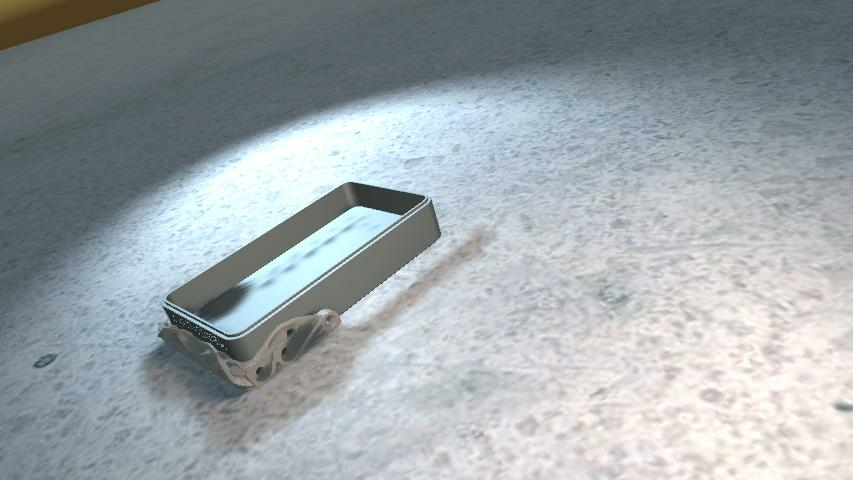
\includegraphics[width=0.5\columnwidth]{figures/sanitizer/unity1.png}
  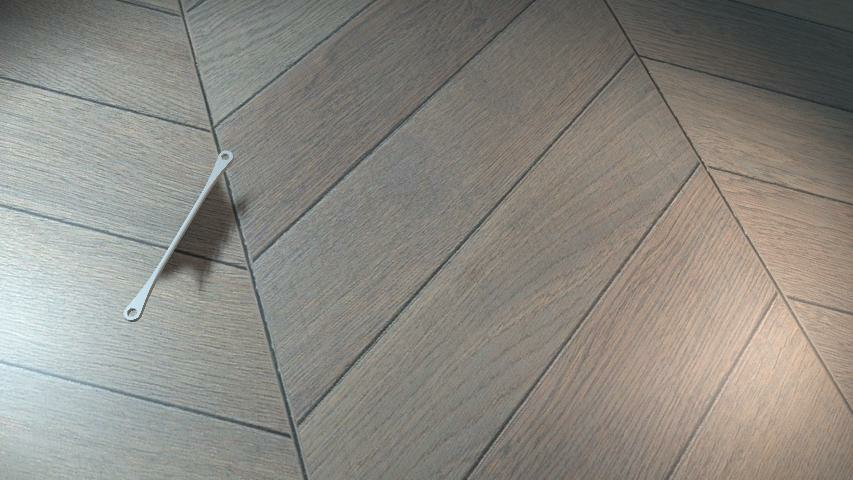
\includegraphics[width=0.5\columnwidth]{figures/sanitizer/unity2.png}
  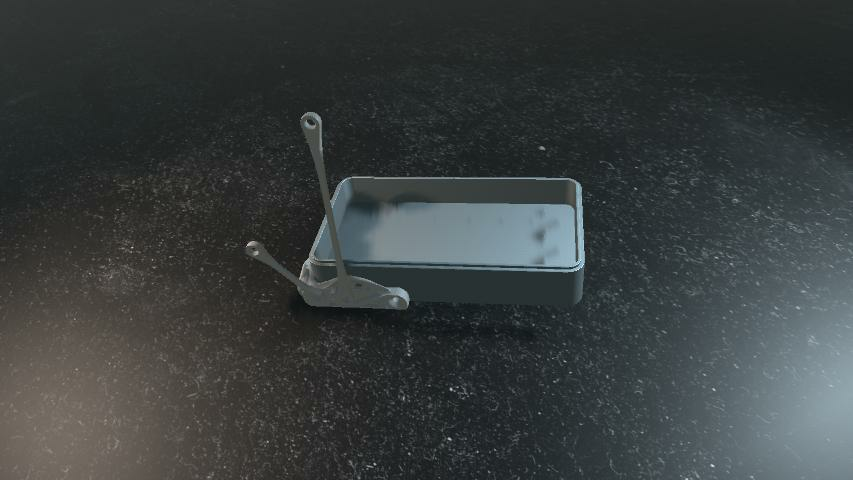
\includegraphics[width=0.5\columnwidth]{figures/sanitizer/unity3.png}
  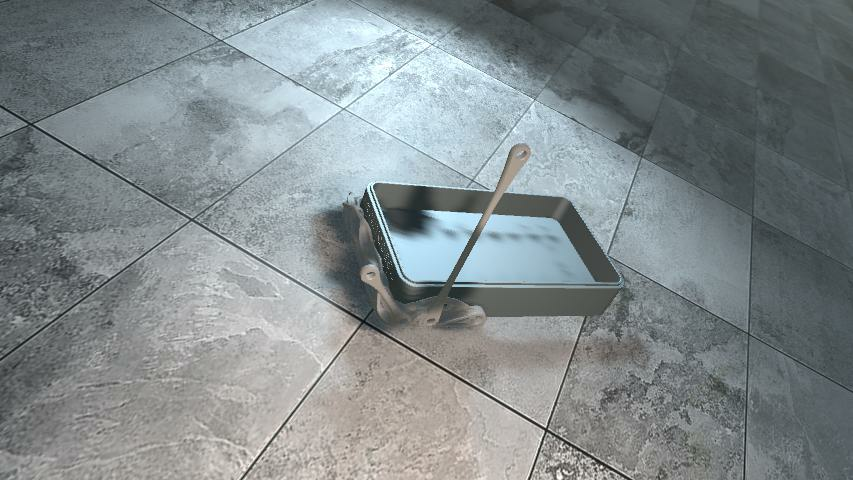
\includegraphics[width=0.5\columnwidth]{figures/sanitizer/unity4.png}
  \caption{
    Synthetic images of the phone sanitizer, from the Unity Perception Package
  }\label{fig:sanitizer_unity}
\end{figure}

\begin{figure}
  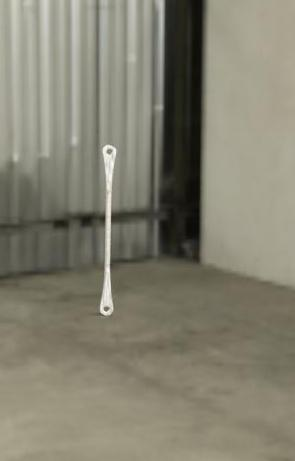
\includegraphics[width=0.5\columnwidth]{figures/sanitizer/a3d1.jpg}
  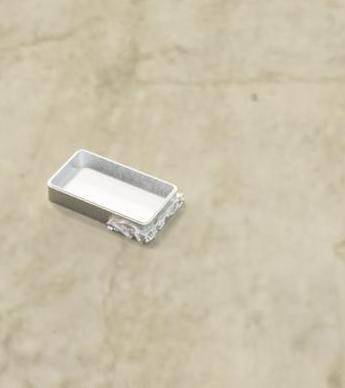
\includegraphics[width=0.5\columnwidth]{figures/sanitizer/a3d2.jpg}
  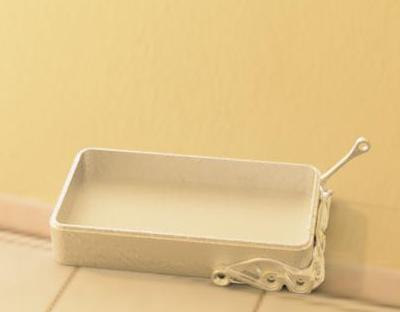
\includegraphics[width=0.5\columnwidth]{figures/sanitizer/a3d3.jpg}
  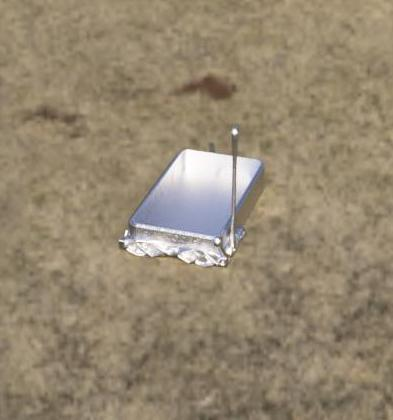
\includegraphics[width=0.5\columnwidth]{figures/sanitizer/a3d4.jpg}
  \caption{
    Synthetic images of the phone sanitizer, from Autodesk A3D
  }\label{fig:sanitizer_a3d}
\end{figure}

\begin{table}[h]
\begin{tabular}{|l||l|l|}
  \hline
  & Unity & A3D\\
  \hline
  \hline
  12,500 & 75\% & 89.6\% \\
  \hline
  25,000 & 81.2\% & 91.6\%\\
  \hline
  50,000 & 85\% & 92.9\%\\
  \hline
\end{tabular}
\begin{captiontext}
    The top row of the table indicates the software used to create the dataset.
    The left column of the table indicates the size of the training set.
    The values in the table are the percentage of our 60,129 test images that
    the pipeline of models classified correctly.
  \end{captiontext}
  \caption{
    Classification results for model pairs trained on data for the phone
    sanitizer
  }\label{tab:sanitizer_accuracy}
  \vspace{-0.1in}
\end{table}

The textures of the sanitizer parts in the A3D images were more realistic than
the textures of the parts in the Unity images.
In particular, the metal surfaces in the A3D images reflect light more
accurately than the metal surfaces in the Unity images.
We hypothesized that the realistic textures were responsible for A3D images
resulting in models that were more accurate than the Unity images.
To verify this hypothesis, we generated a set of images using A3D that used much
simpler textures.
Figure~\ref{fig:sanitizer_a3d_simple} shows examples of these images.
We created three different sized training sets using these images.
Table~\ref{tab:sanitizer_accuracy_simple_textures} lists the accuracies of
models trained on these sets, tested on the test set of real images.
The accuracy was considerably lower than the models trained on our original A3D
dataset, with the same number of images.
This supports our hypothesis that realistic textures were responsible for
the superior performance of the models trained on the A3D images, when
compared with model pairs trained on Unity images.

The model pair trained on 12,500 images was 0.5\% more accurate than the model
pair trained on 25,000 images.
This is a very small difference in performance, but it is unexpected.
One possible explanation for this difference is that the 25,000 image dataset
contained a set of particularly problematic images that were not in the 12,500
image dataset.
The images might have been problematic due to lighting or orientation of the
subassembly.
These problematic images might have eliminated any benefit that the larger
dataset offered.
The model pair trained on 50,000 images was more accurate than either of the
model pairs that were trained on smaller datasets.

\begin{figure}
  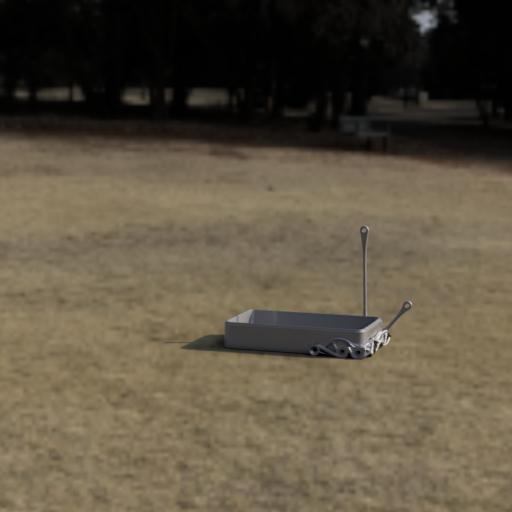
\includegraphics[width=0.33\columnwidth]{figures/synthetic/simple1.jpg}
  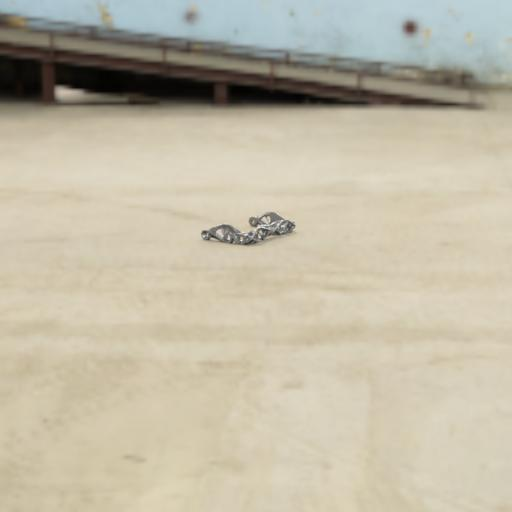
\includegraphics[width=0.33\columnwidth]{figures/synthetic/simple2.jpg}
  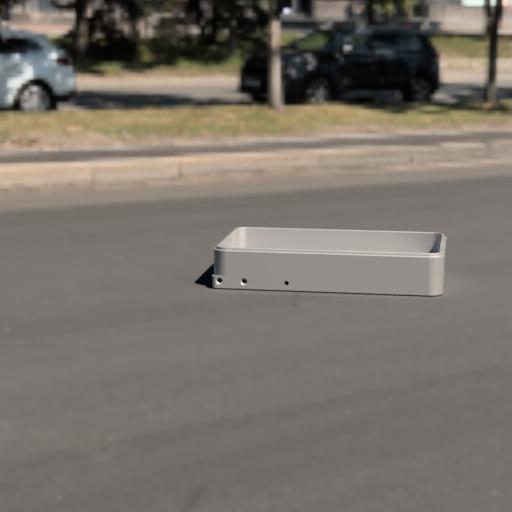
\includegraphics[width=0.33\columnwidth]{figures/synthetic/simple3.jpg}
  \caption{
    Images generated using A3D with simple object textures
  }\label{fig:sanitizer_a3d_simple}
\end{figure}

\begin{table}[h]
\begin{tabular}{|l|l|}
  \hline
  Dataset Size & Accuracy\\
  \hline
  \hline
  12,500 & 77.3\%\\
  \hline
  25,000 & 76.8\%\\
  \hline
  50,000 & 78.84\%\\
  \hline
\end{tabular}
\begin{captiontext}
  These models pairs were trained on simple texture synthetic images of the
  phone sanitizer from A3D.
  Accuracy is the percentage of our 60,129 test images that the pipeline of
  models classified correctly.
\end{captiontext}
  \caption{
    Classification results for simple texture model pairs
  }\label{tab:sanitizer_accuracy_simple_textures}
\end{table}

\section{Discussion}

Capturing and labeling training images for WCA applications is a time
consuming process.  Using synthetic images is less labor-intensive,
and would simplify development of WCA applications.  We have achieved
promising results with this approach for three different assembly tasks.
These results offer the tantalizing promise that
using synthetic data might eliminate the need to manually capture and label
images in order to develop WCA applications for assembly tasks.

\citet{Wang_2022_CVPR} note several ways that A3D could be improved to make
images look better.
The first change they propose is increasing the variation in how objects are
positioned.
Currently, Auto3D renders all objects in a scene with a single texture.
\citet{Wang_2022_CVPR} propose an improvement that would allow parts to be
rendered with different textures.
In addition, \citet{Wang_2022_CVPR} propose to increase the variation in camera
positions used to render the scene.
We believe that all of these proposed changes, especially the improvements to
camera positioning, could result in better training data for the types of
computer vision models that we use.
In addition, software tools liked Autodesk A3D and the Unity Perception package
can be made easier to use.
A developer must create individual CAD files for each step of a task.
For example, if the models must recognize a certain kit with a screw
inserted and without that screw inserted, the developer must create a CAD file
showing the kit before this screw is removed and another CAD file showing the
kit after this screw is removed.
Open Workflow Editor allows a developer to specify a task using a flowchart.
Adding the ability to specify the parts of a CAD model that get inserted or
removed during a task step would make it easier to develop
WCA applications for kits that are born digitally.
In addition, integrating tools for automatic Assembly sequence
planning~\cite{subassembly_identification} into these programs would improve WCA
application development.

After a developer has generated synthetic images, the number of manual steps
required to achieve a working WCA application is still very high.
Autodesk A3D and the Unity Perception package both output annotations in
different formats.
The developer must convert these into the format used by the TensorFlow Object
Detection API, and create another copy in the format used by the Fast MPN-COV
implementation.
Afterwards, the developer must start training object detectors and fine-grained
images classifiers needed by the application.
The developer must then create a flowchart in Open Workflow Editor that
specifies the task instructions and the models that should be used at each step
of the task.
\hl{
  We are actively working to simplify this process by automating the workflow
  of transformations.
}

\chapter{Escalation to Human Experts}\label{chap:escalation}

The techniques presented in the previous chapters allow WCA applications to
detect states that the developer trains models to handle.
The developer can provide example images of the object after each step has been
done correctly.
However, there are many possible ways that an object can be put together
incorrectly.
It is not possible to collect images of every mistake that someone completing a
task might make.
People using these
applications in the real world are going to reach some states that the models
were not trained for. As Dr. Reynold Xin once said,
``A machine learning model is only as good as the data it is fed~\cite{xin}.''
Our models can signal to our application that an image ``looks most similar to
this set of images from the training data.''
These models are not capable of a more general understanding, such as ``the long
brass piece is screwed on upside down.''

Detecting all possible error states would require us to have examples of these
states in our training data. There is a combinatorial explosion in the number of
error states, compared to the number of correct states, so collecting training
data for every possible error is not practical.
Instead, we handle errors that our models were not trained to recognize by
having people completing tasks call a human expert from the application.
The user's camera feed during these calls can be recorded, and these recordings
can provide data to train models to recognize these errors in the future.
This allows us to follow a DevOps strategy when developing these applications.
A team of developers can launch an initial version of a WCA application that
detects a small number of error states.
As the application gets used, and people call in to get help with new errors,
the developers can improve the application to detect these errors.
Over time, this process will increase the number of error states that our
application can detect.

\section{Experts Without Automation}

Several commercial products allow a remote human expert to help a user through
an assembly task.
Examples of such systems include Microsoft Dynamics 365 Remote
Assist~\cite{dynamics365}, Webex Expert on Demand~\cite{webex},
AMA XpertEye~\cite{xpert}, and Vieaura~\cite{vieaura}.
The person completing the task wears a headset with a camera, but the expert
must be on a call with a single user for the duration of an entire task.
A task expert's time is valuable.
We believe that integrating wearable cognitive assistance with
human assistance will allow products like these to scale from requiring
experts to work one on one through each step of the task to enabling experts to
help multiple users concurrently.

\section{Calls With Human Experts}

The computer vision models that our applications use are not perfect. In order
to handle cases where a model makes a mistake, our applications allow the user
to start a call with a human who is an expert on the task being completed. The
human expert sees a feed from the user's camera and they can talk the user
through correcting problems. In addition, the expert can change the step that
the application thinks the user is in the middle of, and then the user can
continue to receive guidance from the application after the call ends.
The application can also be modified to suggest calling the expert, if a user
has been stuck on a step for a certain amount of time.
However, additional research is required to determine what should trigger a
suggestion to call the expert.
Potential options include triggering a suggestion after the application has seen
a sequence of frames with identical perceptual hash
values, or simply a certain amount of time passing without the user advancing a
step.
In addition, it might not be necessary to suggest calling the expert in the
first place, as users have the option to start the call at any point.
Figure~\ref{fig:design_space} shows options for task guidance systems that use
human experts.

\begin{figure}[H]
  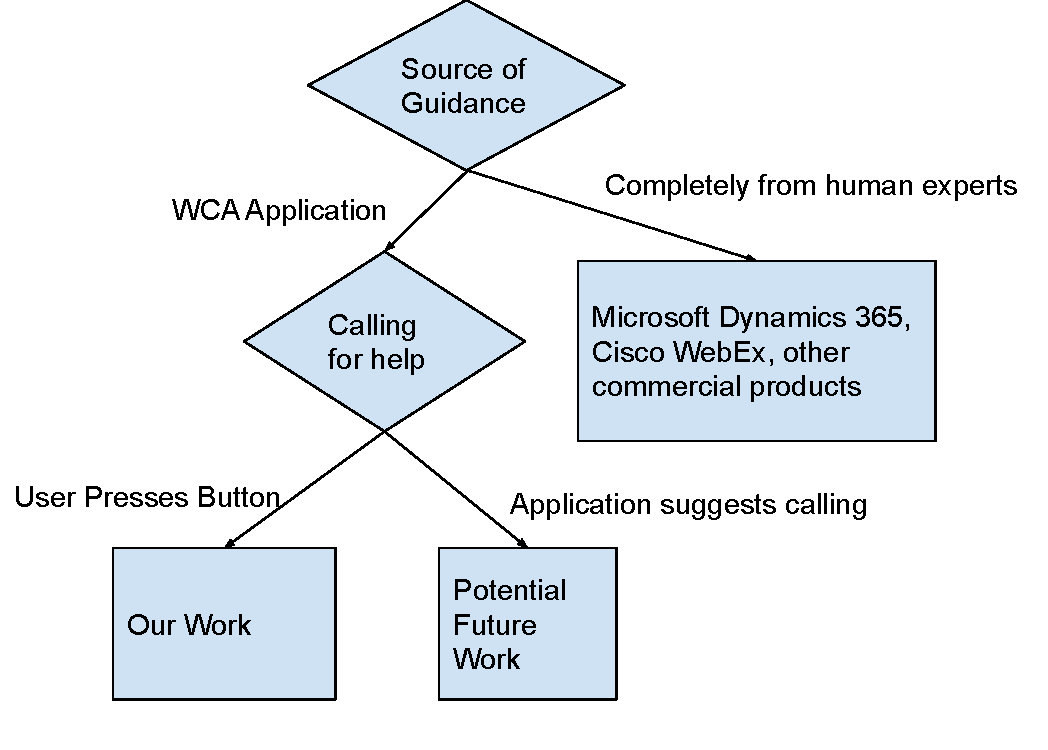
\includegraphics[width=14cm]{figures/design_space.pdf}
  \caption{The design space for systems that allow experts to remotely help with
    assembly tasks.
    Our system primarily guides users with a WCA application.
    Users must explicitly press a button to start a call with a human expert.
  }\label{fig:design_space}
\end{figure}

When we train models for Gabriel applications, we consider each state of a task
to be one object. Open World Object Detection~\cite{joseph2021open} is an active
area of research into models that can learn to detect previously unlabeled
objects. However, this does not help with recognizing such an object the first
time it is seen. Gabriel applications need to handle all errors, even ones that
have not been seen before. A human who is an expert on the task can do this.

Correcting error states in Gabriel applications can be done on the order of tens
of seconds to a few
minutes, unlike driving a car which might require sub-second response times.
It's perfectly acceptable for the user to press a button to call for help from
an expert, if the application does not detect that a step has been completed
after a certain amount of time. The user will then be connected to someone who
is an expert on this task. The expert will
see the camera feed from the headset and talk back and forth with the user to
help them get back to a state that the computer vision models can handle.
The expert will also have the ability to update the application's state, so the
user can continue receiving automated guidance from an earlier or later
step after the call.
This workflow is depicted in Figure~\ref{fig:zoom_workflow}.

\begin{figure}[H]
  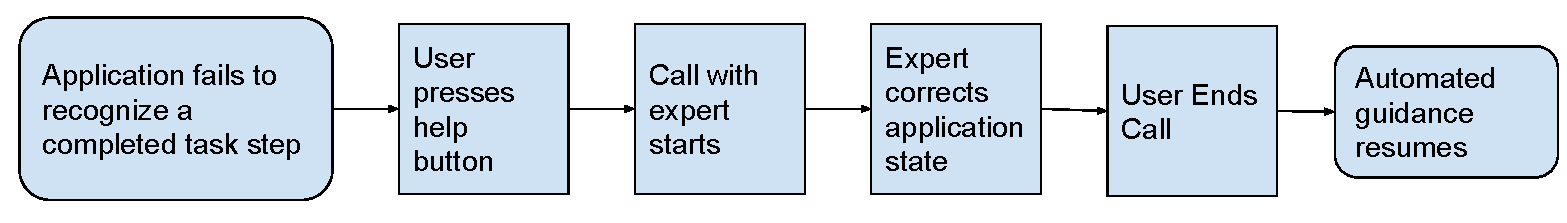
\includegraphics[width=\textwidth]{figures/zoom_workflow.pdf}
  \caption{The workflow followed by a WCA application user requesting help from
    a human expert.
  }\label{fig:zoom_workflow}
\end{figure}

We connect users to task experts using Zoom, which offers SDKs for several
platforms~\cite{Zoom}. The Gabriel user runs an Android application on a
smartphone or Google Glass, which starts a call with the expert using Zoom's
Android SDK.
The human expert uses a web application that incorporates Zoom's Web SDK.
Figure~\ref{fig:expertui} shows a screenshot of this application.
The expert's web application allows them to see the user's camera feed, as well
as the step that the user is currently working on.
The application works for any WCA task that was created with OpenWorkflow
Editor.
The code can be modified to use a different video calling service in the future.
The components of the system are shown in Figure~\ref{fig:expert_components}.

\begin{figure}[H]
  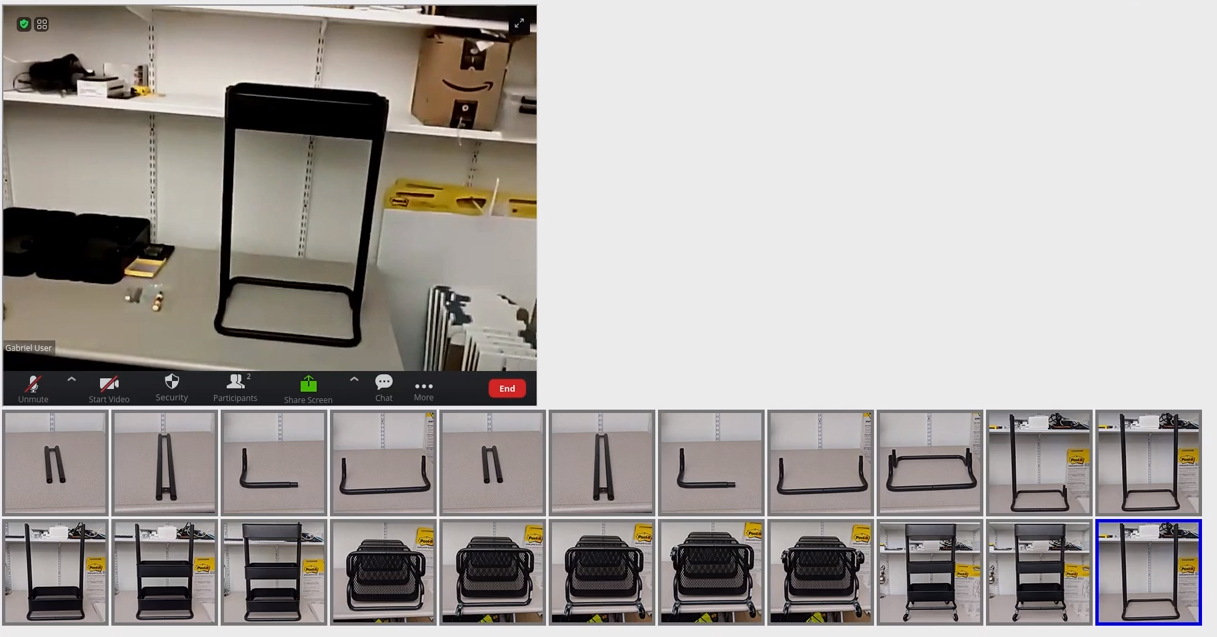
\includegraphics[width=\textwidth]{figures/expert_ui.png}
  \caption{A screenshot of the web application used by the human task expert.
    The feed from the user's camera is shown on top. The task steps are shown on
    the bottom. The step that the application believes the user is currently
    working on is surrounded by the
    blue box. Clicking on a different step will change the current step
    to the one that was clicked on.
  }\label{fig:expertui}
\end{figure}

\begin{figure}[H]
  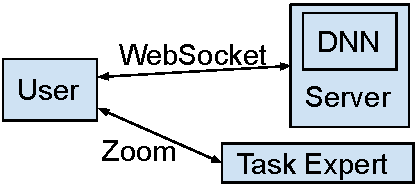
\includegraphics[width=8cm]{figures/human_assitance.pdf}
  \caption{The components of a Gabriel application with human assistance. The
    user primarily receives guidance from a server running a DNN. If the user
    reaches a point where the automated assistance fails, they can switch over
    to receiving guidance from a human expert over a video call.
  }\label{fig:expert_components}
\end{figure}

\section{Simulating Call Centers}

Supporting a large number of people using WCA applications at the same time
would require multiple human experts answering support calls.
It is important to employ enough experts to ensure that wait times are
reasonable.
However, having too many experts working at one time will create unnecessary
expenses.

We developed a simulation that people running a call center for a WCA
application could use to determine the number of experts they should have
available to assist the users who call for help.
A person using our simulation to determine the number of experts that they
should hire will need to provide parameters to the simulation for their specific
task.
We did not have any real data to determine these parameter values, so we made up
values that seemed reasonable based on our experiences developing and using WCA
applications.
However, our code can be easily re-run with different parameter values.

There is a large body of work examining wait times for call
centers~\cite{queue1, queue2}.
Our work is different because we simulate a user completing a task with a WCA
application.
A single user might call the expert multiple times, if they get stuck on
multiple steps.
In addition, we model user patience, to determine the amount of time a user will
wait before calling the expert.

\subsection{Existing Call Center Models}

Kendall's notation is used to describe queuing models, by specifying the arrival
process, the distribution of service times, and the number of
servers~\cite{kendall}.
The arrival process determines how the amount of time between calls to the
expert should be sampled.
The amount of time that a user and an expert spend on a call with each other is
the service time.
The number of servers refers to the number of experts.

M/M/N is an example of Kendall's notation, where the queue has a Poisson arrival
process, a Poisson service time distribution, and more than one server.
The time between events for a Poisson arrival process follows an exponential
distribution.
An exponential distribution has the probability density function
$lambda * e ^ {- lambda x}$ when x is above 0.
As shown in Figure~\ref{fig:simple_sim1_dists}, it takes the form of a
negatively accelerated decreasing function of x, where the rate of decrease is
governed by $lambda$.
This model is simulated in Section~\ref{sec:simple}.

The M/M/N model (Erlang-C) is often used to model call centers~\cite{queue1}.
This model assumes that call service times are exponentially distributed.
However, two studies of logs from actual call centers have shown service times
to be lognormally distributed~\cite{queue1, queue2}.
A normal distribution follows a bell curve, with mean $\mu$ and standard
deviation $\sigma$.
If a variable, $X$, is lognormally distributed, $\ln{(X)}$ is lognormally
distributed.
Figure~\ref{fig:simple_sim2_dists} shows an example of a probability density
function for a lognormal distribution.

The probability density function for a lognormal distribution is:
\[
  \frac{1}{x \sigma \sqrt{2 \pi}}
  \exp{\left( - \frac{\left( \ln(x) - \mu \right)^2}{2 \sigma^2} \right)}
\]


Lognormal service times require an M/G/N model, which has a Poisson arrival
process, more than one server, and allows for any distribution of service times.
Section~\ref{sec:sim_lognormal} simulates this model.
\citet{queue1} examined the expected call center wait time $E(W)$ using the
following approximation for an M/G/N queue:

\begin{equation}
  E(W) \approx \frac{1}{N} \frac{\rho}{1 - \rho} \frac{1 + C_s^2}{2} E(S)
\label{eq:wait}
\end{equation}

Wait time is the period between when a user requests help, and when the user
gets connected to the expert.
We measure this in seconds.
$N$ is the number of experts available in the call center,
$C_s = \sigma_s / E(S)$ is the coefficient of variation for service, and
$E(S)$ and $\sigma_s$ are the mean and standard deviation of service times.
$E(S)$ and $\sigma_s$ are estimated based on the service time values that our
actual simulation samples.

The system occupancy is:
\begin{equation}
\rho = \frac{\lambda}{N \mu}
\label{eq:occupancy}
\end{equation}

$\lambda$ is the arrival rate and $\mu$ is the service rate ($E(S) = 1/µ$).

The M/G/N queue assumes that all call inter-arrival times are independent of
service times and other inter-arrival times.
If a user had the option to give up on waiting, this would violate the
independence assumption.
Our models do not allow the simulated users to give up on waiting.

\subsection{Simple Simulation}\label{sec:simple}

We compared the wait times from Formula~\ref{eq:wait} with a simple Monte Carlo
simulation that obeys the independence assumption, which we will call Simulation
1.
The simulation modeled users calling in, waiting until an expert in the
call center is available to speak, and then the user and the expert are on the
call for a certain amount of time.
There is a single queue for all users waiting for an expert, and it is serviced
in first in, first out (FIFO) order.
An expert will service the next call from the queue as soon as they finish their
current call.
The inter-arrival time between calls coming in was sampled from an exponential
distribution.
The lengths of calls were sampled from an exponential distribution with TODO FIXME
These two distributions are depicted in Figure~\ref{fig:simple_sim1_dists}.
Samples were generated using SciPy~\cite{scipy}.
Unfortunately we did not have any real data to help inform the parameter values
for our distributions.
Therefore, we picked parameter values that seemed reasonable based on our
experiences with WCA applications.
Figure~\ref{fig:simple_sim1_results} shows how the waiting times from our
simulation and the formula vary as we increase the number of experts.
The system occupancy, which is computed according to Formula~\ref{eq:occupancy},
cannot exceed 1.
Otherwise, calls will arrive faster than they can be answered, and the queue
will continue to grow the longer the simulation is run.
We thus only report results for cases where the system occupancy is below 1.

\begin{figure}[H]
  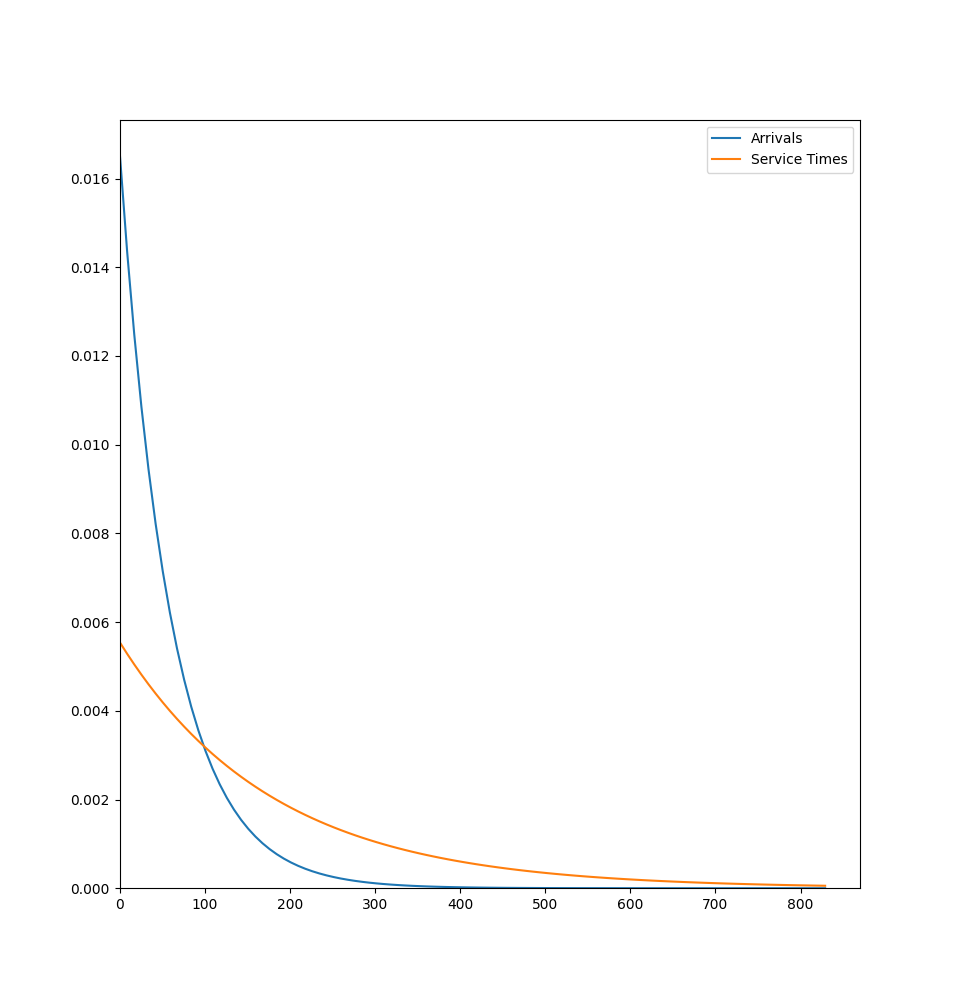
\includegraphics[width=\textwidth]{figures/montecarlo/expon_expon.png}
  \caption{
    The probability density functions (PDFs) for the distributions that
    Simulation 1 sampled times from.
    The inter-arrival times and service times were both sampled from
    exponential distributions.
  }\label{fig:simple_sim1_dists}
\end{figure}

\begin{figure}[H]
  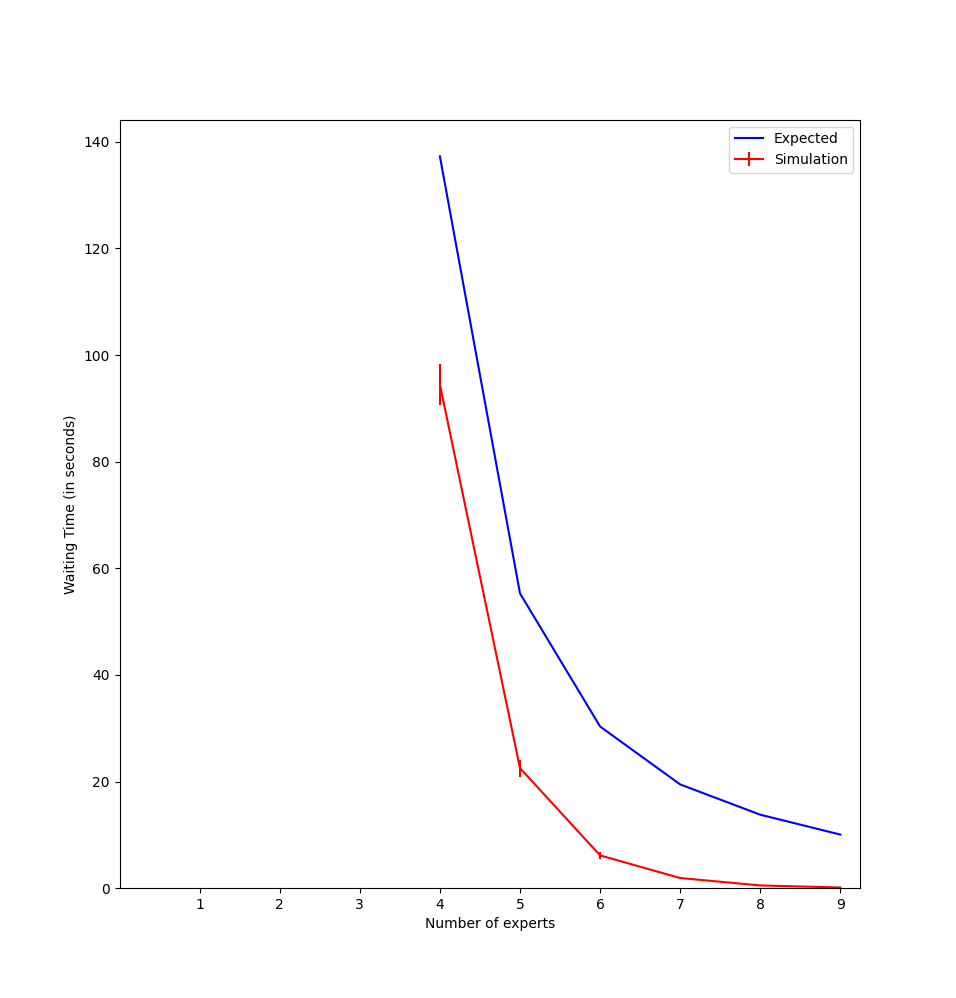
\includegraphics[width=\textwidth]{figures/montecarlo/independent_calls_expon.png}
  \caption{
    The waiting times resulting from Simulation 1 and Formula~\ref{eq:wait}.
    The time values were sampled from the distributions shown in
    Figure~\ref{fig:simple_sim1_dists}.
  }\label{fig:simple_sim1_results}
\end{figure}

\subsection{Lognormal Service Times}\label{sec:sim_lognormal}

Two studies of logs from actual call centers observed that distributions of
service times were lognormal~\cite{queue1, queue2}.
We therefore modified our simulation to sample call lengths from a lognormal
distribution, but we kept the exponential distribution for inter-arrival time
samples.
We will refer to this version of the simulation as Simulation 2.
We ran the simulation with different numbers of experts.
The experiment was repeated 10 times, with different random values, for each
setting of the number of experts.
The number of users completing the task at any given point is a function of the
Poisson arrival process described in \S\ref{sec:simple}, and the lengths of time
that it takes users to complete the full task.
The distributions for Simulation 2 are depicted in
Figure~\ref{fig:simple_sim2_dists}.
The results from the simulation and Formula~\ref{eq:wait} are shown in
Figure~\ref{fig:simple_sim2_results}.
The waiting time from the formula was higher than the waiting time from
the simulation in every case.
We believe this difference is due to the fact that the formula is just an
approximation.
In addition, the formula is approximating a queue with an arbitrary probability
distribution for service times.
Thus it is more general than our simulation, which specifically uses a lognormal
distribution for service times.

\begin{figure}[H]
  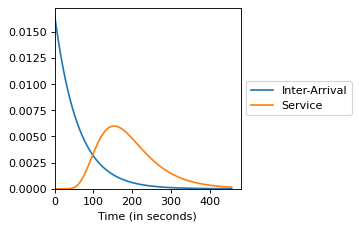
\includegraphics[width=\textwidth]{figures/montecarlo/expon_lognorm.png}
  \caption{
    The PDFs for the distributions that Simulation 2
    sampled times from.
    The inter-arrival times were sampled from an exponential distribution.
    The service times were sampled from a lognormal distribution.
  }\label{fig:simple_sim2_dists}
\end{figure}

\begin{figure}[H]
  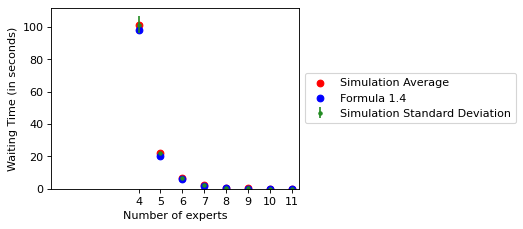
\includegraphics[width=\textwidth]{figures/montecarlo/independent_calls_lognorm.png}
  \caption{
    The waiting times resulting from Simulation 2 and Formula~\ref{eq:wait}.
    The time values were sampled from the distributions shown in
    Figure~\ref{fig:simple_sim2_dists}.
  }\label{fig:simple_sim2_results}
\end{figure}

\subsection{Simulating All Steps}

We expanded our simulation to model users completing an entire task with a WCA
application.
We will refer to this version as Simulation 3.
Rather than starting at the point that a call comes into the call center, we
also model users receiving automated guidance and calling for help if they get
stuck.
The simulation includes user patience, which is the amount of time a person is
willing to spend on a step, before they give up and call the expert.
Most steps of the task will be possible.
This means that a user will eventually complete the step if they spend enough
time on it.
However, a user's patience is finite.
In addition, some steps might be impossible, which means that the user cannot
complete them without calling the expert.
Impossible steps could be a result of incorrectly manufactured parts, bad
lighting, or poorly trained machine learning models.
It is therefore in the user's best interest to give up on a step and call the
expert at some point.

Inter-arrival times for users starting the task are sampled from an exponential
distribution.
The simulation models users completing the task according to the process
described in Figure~\ref{algo:sim}.
This process is repeated for each simulated user.
The simulation allows users to work in parallel.
However, if a user calls for help while all experts are busy, they must wait in
a queue for service.
As in the previous simulations, all users wait in a single queue that is
serviced in FIFO order.

\begin{algorithm}[H]
  \For{Step in task}{
    sample patience length\;
    sample step possibility\;
    \eIf{step possibility is 1}{
      sample step length\;
      \eIf{step length < patience length}{
        Pause for step length\;
        User completes step successfully\;
      }{
        Pause for patience length\;
        User calls expert for help\;
        }
      }{
        Pause for patience length\;
        User calls expert for help\;
    }
  }
  \caption{
    The process used to simulate one user completing a task using a WCA
    application.
  }\label{algo:sim}
\end{algorithm}

Simulation 3 samples from distributions used in existing literature.
Patience length is sampled from a generalized Pareto distribution.
\citet{patience} found a generalized Pareto distribution to be a good fit for
samples of time that people waited before crossing streets, while the crossing
signal was telling them not to cross.
Step possibility was sampled from a Bernoulli distribution.
Step length was sampled from an exponentially modified Gaussian distribution.
\citet{dawson1988fitting} suggested modeling response times from an
exponentially modified Gaussian distribution.
Figure~\ref{fig:step_patience} shows the generalized Pareto and exponentially
modified Gaussian distributions that were used.

When the sampled step possibility value is 1, and the patience length value is
smaller than the step length value, the user will call the expert for help.
This represents a user giving up on a step that is possible.
One can increase the fraction of steps that a user will give up on by shifting
the step length distribution to the right and/or shifting the patience length
distribution to the left.

\begin{figure}[H]
  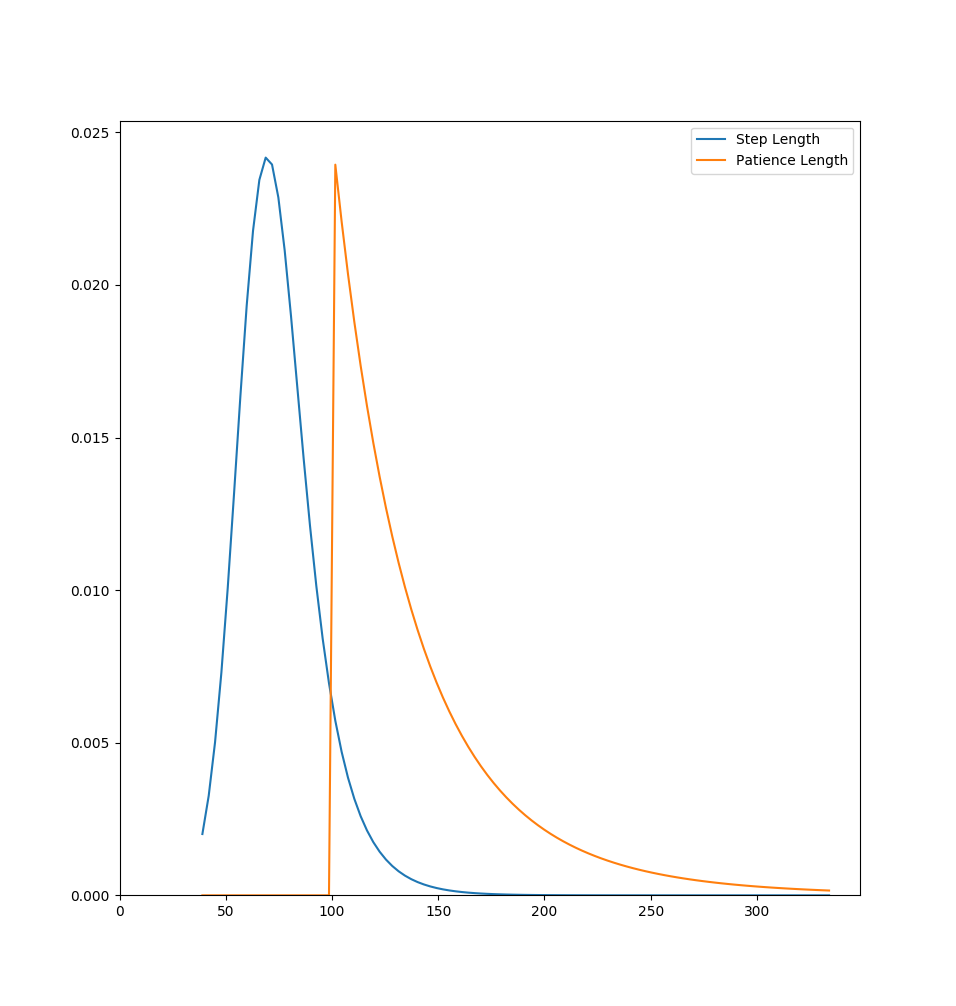
\includegraphics[width=\textwidth]{figures/montecarlo/step_patience.png}
  \caption{
    The PDFs for the generalized Pareto distribution that our simulation samples
    patience length from, and the exponentially modified Gaussian distribution
    that our simulation samples step length from.
    Sampling from these distributions resulted in users giving up on about 2.5\%
    of possible steps.
  }\label{fig:step_patience}
\end{figure}

The samples from the exponential distribution that were used to determine
Inter-arrival times for users starting the task are shown in
Figure~\ref{fig:arrival_times}.
The times at which a user in our simulation called for help are shown in
Figure~\ref{fig:step_patience}.
We fit an exponential curve to both of these sets of data.
The $R^2$ for the exponential fit was 0.991 for the inter-arrival times of users
starting the task, and 0.986 for the inter-arrival times of users calling for
help.

\begin{figure}[H]
  \includegraphics[width=\textwidth]{figures/montecarlo/arrival_times.png}
  \caption{
    Our inter-arrival time samples for users starting the task are shown in
    blue.
    These were drawn from an exponential distribution.
    We fit an exponential curve to this data, which is shown in red.
  }\label{fig:arrival_times}
\end{figure}

\begin{figure}[H]
  \includegraphics[width=\textwidth]{figures/montecarlo/call_times.png}
  \caption{
    The inter-arrival times for help calls that resulted from Simulation 3.
    We fit an exponential curve to this data, which is shown in red.
  }\label{fig:step_patience}
\end{figure}

\subsubsection{Servicing Calls}

Our simulation sampled call lengths from a lognormal distribution.
The average waiting time for users in our simulation is shown in
Figure~\ref{fig:full_expected_sim}, along with the expected waiting times from
Formula~\ref{eq:wait}.
There was a huge variation in waiting time across different runs of the
simulation with five experts.
However, this variation decreased substantially when we ran the simulation with
six users.
This makes sense intuitively, as there was more of a buffer to handle bursts of
calls coming in.
The average wait time across runs of Simulation 3 with five experts was 31.3\%
higher than the expected wait time from Formula~\ref{eq:wait}.
With six users, the time from Formula~\ref{eq:wait} was 45.1\% higher than the
average time from Simulation 3.
The times from Formula~\ref{eq:wait} were 77.7\%, 180.3\%, and 646.1\% higher
than the average time from Simulation 3, for 7, 8, and 9 users
respectively.

\begin{figure}[H]
  \includegraphics[width=\textwidth]{figures/montecarlo/full_expected_sim.png}
  \caption{
    The average waiting time for simulated users, and the expected waiting time
    for an M/G/N queue.
  }\label{fig:full_expected_sim}
\end{figure}

The simulation results are plotted against the times from Formula~\ref{eq:wait}
in Figure~\ref{fig:gof}.
Fitting a linear model to these values achiever an $R^2$ coefficient of 0.96.
This strong fit indicates that the waiting times from the simulation have a
linear relationship to the waiting times from the formula.

\begin{figure}[H]
  \includegraphics[width=\textwidth]{figures/montecarlo/gof.png}
  \caption{
    The average waiting time for simulated users plotted against expected
    waiting times from Formula~\ref{eq:wait}.
  }\label{fig:gof}
\end{figure}

WCA applications can send details to the call center about how long a person has
been stuck on a step, or how long the person has spent on the task overall.
We ran versions of our simulation with two alternative orderings for servicing
calls, to see if this additional information might reduce the overall average
waiting times.
The first alternative ordering served the user in the queue who has completed
the largest number of steps first.
The next ordering prioritized the user who had been stuck on a step for the
largest amount of time.
In particular, a user who spent three minutes trying to complete a step, and
then
called the expert one minute ago would get serviced before a user who spent one
minute trying to complete a step, and then called the expert two minutes ago.
A comparison of these queuing strategies is shown in
Figure~\ref{fig:full_three_strategies}.
The results were nearly identical with all three strategies.
Given the difficulty of implementing these alternative orderings in a real
system, we feel that servicing calls in FIFO order is sufficient.

\begin{figure}[H]
  \includegraphics[width=\textwidth]{figures/montecarlo/full_three_strategies.png}
  \caption{
    A comparison of simulation results, with three different queuing strategies.
  }\label{fig:full_three_strategies}
\end{figure}

Our code was written in a way that makes it easy to change the distributions
that our simulation samples values from, or the parameters of these
distributions.
An organization running a call center for a WCA application can collect data
based on people using this application.
They can then run Simulation 3 with these values, and see expected wait times
for different numbers of experts.
This will tell them the number of experts that they should hire in order to keep
wait times in their call center acceptable.

\section{Exploring Parameter Space}

This simulation allows us to see how average wait time changes, when we modify
one variable, and leave all other variables constant.

We ran these simulations with nine experts.
We sample from the same distributions used in Simulation 3.
The simulation was run ten times for each variable value we tested.

\subsection{Varying the Fraction of Possible Steps}

This experiment varied the fraction of steps that the user had the ability to
complete.
A possible step is one that a user can complete if they spend enough time on it.
However, a user might choose to give up and call the expert before the step is
complete.
An impossible step cannot be completed unless the user calls the expert.
Results are shown in Figure~\ref{fig:vary_success}.
As the fraction of impossible steps increases, the average waiting time
increases.
This is because an increase in the number of impossible steps will increase the
number of calls to the expert.

\begin{figure}[H]
  \includegraphics[width=\textwidth]{figures/montecarlo/vary_success.png}
  \caption{
    The average wait time that resulted from changing the fraction of possible
    steps.
  }\label{fig:vary_success}
\end{figure}

\subsection{Varying Patience Length}

Patience length is the amount of time that a user is willing to spend trying to
complete a step, before calling the expert.
The average waiting time that resulted from different average lengths of
patience are shown in Figure~\ref{fig:vary_patience}.
Increasing average patience length reduces the number of calls users will make
to the expert.
Thus the average waiting time decreases as average patience length increases.

\begin{figure}[H]
  \includegraphics[width=\textwidth]{figures/montecarlo/vary_patience.png}
  \caption{
    The average wait time that resulted from changing the amount of users'
    simulated patience.
  }\label{fig:vary_patience}
\end{figure}

\subsection{Varying Length of Possible Steps}

This experiment varied the average amount of time that a user must spend in
order to complete a possible step.
Figure~\ref{fig:vary_step_length} shows the results of this.
Increasing average step length increases the likelihood that a step will take
longer than a user's patience length.
This results in more calls being made to the expert.
Therefore, increasing average step length increases the average waiting time.

\begin{figure}[H]
  \includegraphics[width=\textwidth]{figures/montecarlo/vary_step_length.png}
  \caption{
    The average wait time that resulted from changing the average amount of time
    it took to complete a possible step.
  }\label{fig:vary_step_length}
\end{figure}


\backmatter

%\renewcommand{\baselinestretch}{1.0}\normalsize

% By default \bibsection is \chapter*, but we really want this to show
% up in the table of contents and pdf bookmarks.
\renewcommand{\bibsection}{\chapter{\bibname}}
%\newcommand{\bibpreamble}{This text goes between the ``Bibliography''
%  header and the actual list of references}
\bibliographystyle{plainnat}
\bibliography{thesis} %your bib file

\end{document}
